\documentclass[twoside]{book}

% Packages required by doxygen
\usepackage{fixltx2e}
\usepackage{calc}
\usepackage{doxygen}
\usepackage[export]{adjustbox} % also loads graphicx
\usepackage{graphicx}
\usepackage[utf8]{inputenc}
\usepackage{makeidx}
\usepackage{multicol}
\usepackage{multirow}
\PassOptionsToPackage{warn}{textcomp}
\usepackage{textcomp}
\usepackage[nointegrals]{wasysym}
\usepackage[table]{xcolor}

% Font selection
\usepackage[T1]{fontenc}
\usepackage[scaled=.90]{helvet}
\usepackage{courier}
\usepackage{amssymb}
\usepackage{sectsty}
\renewcommand{\familydefault}{\sfdefault}
\allsectionsfont{%
  \fontseries{bc}\selectfont%
  \color{darkgray}%
}
\renewcommand{\DoxyLabelFont}{%
  \fontseries{bc}\selectfont%
  \color{darkgray}%
}
\newcommand{\+}{\discretionary{\mbox{\scriptsize$\hookleftarrow$}}{}{}}

% Page & text layout
\usepackage{geometry}
\geometry{%
  a4paper,%
  top=2.5cm,%
  bottom=2.5cm,%
  left=2.5cm,%
  right=2.5cm%
}
\tolerance=750
\hfuzz=15pt
\hbadness=750
\setlength{\emergencystretch}{15pt}
\setlength{\parindent}{0cm}
\setlength{\parskip}{3ex plus 2ex minus 2ex}
\makeatletter
\renewcommand{\paragraph}{%
  \@startsection{paragraph}{4}{0ex}{-1.0ex}{1.0ex}{%
    \normalfont\normalsize\bfseries\SS@parafont%
  }%
}
\renewcommand{\subparagraph}{%
  \@startsection{subparagraph}{5}{0ex}{-1.0ex}{1.0ex}{%
    \normalfont\normalsize\bfseries\SS@subparafont%
  }%
}
\makeatother

% Headers & footers
\usepackage{fancyhdr}
\pagestyle{fancyplain}
\fancyhead[LE]{\fancyplain{}{\bfseries\thepage}}
\fancyhead[CE]{\fancyplain{}{}}
\fancyhead[RE]{\fancyplain{}{\bfseries\leftmark}}
\fancyhead[LO]{\fancyplain{}{\bfseries\rightmark}}
\fancyhead[CO]{\fancyplain{}{}}
\fancyhead[RO]{\fancyplain{}{\bfseries\thepage}}
\fancyfoot[LE]{\fancyplain{}{}}
\fancyfoot[CE]{\fancyplain{}{}}
\fancyfoot[RE]{\fancyplain{}{\bfseries\scriptsize Generated by Doxygen }}
\fancyfoot[LO]{\fancyplain{}{\bfseries\scriptsize Generated by Doxygen }}
\fancyfoot[CO]{\fancyplain{}{}}
\fancyfoot[RO]{\fancyplain{}{}}
\renewcommand{\footrulewidth}{0.4pt}
\renewcommand{\chaptermark}[1]{%
  \markboth{#1}{}%
}
\renewcommand{\sectionmark}[1]{%
  \markright{\thesection\ #1}%
}

% Indices & bibliography
\usepackage{natbib}
\usepackage[titles]{tocloft}
\setcounter{tocdepth}{3}
\setcounter{secnumdepth}{5}
\makeindex

% Hyperlinks (required, but should be loaded last)
\usepackage{ifpdf}
\ifpdf
  \usepackage[pdftex,pagebackref=true]{hyperref}
\else
  \usepackage[ps2pdf,pagebackref=true]{hyperref}
\fi
\hypersetup{%
  colorlinks=true,%
  linkcolor=blue,%
  citecolor=blue,%
  unicode%
}

% Custom commands
\newcommand{\clearemptydoublepage}{%
  \newpage{\pagestyle{empty}\cleardoublepage}%
}

\usepackage{caption}
\captionsetup{labelsep=space,justification=centering,font={bf},singlelinecheck=off,skip=4pt,position=top}

%===== C O N T E N T S =====

\begin{document}

% Titlepage & ToC
\hypersetup{pageanchor=false,
             bookmarksnumbered=true,
             pdfencoding=unicode
            }
\pagenumbering{roman}
\begin{titlepage}
\vspace*{7cm}
\begin{center}%
{\Large My Project }\\
\vspace*{1cm}
{\large Generated by Doxygen 1.8.11}\\
\end{center}
\end{titlepage}
\clearemptydoublepage
\tableofcontents
\clearemptydoublepage
\pagenumbering{arabic}
\hypersetup{pageanchor=true}

%--- Begin generated contents ---
\chapter{Projet C++}
\label{md__home_gregory_Desktop_Cours_EK_P2_Pages_projet_test_git_proba_num_README}
\hypertarget{md__home_gregory_Desktop_Cours_EK_P2_Pages_projet_test_git_proba_num_README}{}
Etudier le schéma d’ordre faible élevé introduit dans \mbox{[}1\mbox{]} et étendu dans \mbox{[}2\mbox{]} pour les modèles affines.
\begin{DoxyItemize}
\item Appliquer cette méthode pour le pricing d’options asiatiques dans le modèle de Heston. Comparer avec différentes méthodes de réduction de variance.
\item Comment mettre en œuvre cette méthode dans le cadre Quasi-\/\+Monte Carlo ? Tester numériquement.
\end{DoxyItemize}

\mbox{[}1\mbox{]} S. Ninomiya and N. Victoir. Weak approximation of stochastic differential equations and application to derivative pricing. Appl. Math. Finance, 15(1-\/2) \+:107–121, 2008. \mbox{[}2\mbox{]} A. Alfonsi. High order discretization schemes for the cir process \+: Application to affine term structure and heston models. Math. Comput., 79(269) \+:209–237, 2010.

\href{https://github.com/Gregory-Calvez/proba_num}{\tt https\+://github.\+com/\+Gregory-\/\+Calvez/proba\+\_\+num}

\subsection*{Prérequis}

Ce projet utilise principalement la S\+TL du C++11. Certains éléments doivent être installés pour reproduire tous les graphes et résultats du rapport.
\begin{DoxyItemize}
\item G\+N\+Uplot. Les graphes sont générés à partir de G\+N\+Uplot. \href{http://www.gnuplot.info/}{\tt http\+://www.\+gnuplot.\+info/}
\item G\+SL. G\+NU Scientific Library. \href{https://www.gnu.org/software/gsl/}{\tt https\+://www.\+gnu.\+org/software/gsl/}
\item N\+V\+I\+D\+IA Toolkit. \href{https://developer.nvidia.com/cuda-downloads?target_os=Linux&target_arch=x86_64&target_distro=Ubuntu&target_version=1604&target_type=runfilelocal}{\tt https\+://developer.\+nvidia.\+com/cuda-\/downloads?target\+\_\+os=\+Linux\&target\+\_\+arch=x86\+\_\+64\&target\+\_\+distro=\+Ubuntu\&target\+\_\+version=1604\&target\+\_\+type=runfilelocal}. Les calculs sur G\+PU du rapport ont été faits avec la version 8.\+0 du Toolkit N\+V\+I\+I\+DA pour des raisons de compatibilités avec le G\+PU. Tout devrait fonctionner avec le Toolkit le plus récent.
\end{DoxyItemize}

\subsection*{Structure du projet et compilation}

\subsubsection*{Structure du projet}

Le projet se sépare en deux parties distinctes\+:
\begin{DoxyItemize}
\item une partie reposant sur la programmation orientée objet en C++. Les sources sont disponibles dans le dossier src/
\item une partie reposant sur du calcul parallélisé en C\+U\+D\+A/C. Tout est regroupé dans le dossier cuda/
\end{DoxyItemize}

Un makefile, rédigé à la main, comprend toutes les commandes nécessaires pour reproduire les résultats du rapport.

Des fichiers annexes sont présents, pour les tracés des graphes notamment. Enfin, nous avons conservé dans le dossier du projet des outputs de la console (output/) et des graphes générés (img/) que nous avons réutilisés dans le rapport.

Une documentation de la partie C++ réalisée avec Doxygen est disponible dans le dossier doc/.

\subsubsection*{Compilation}

Dans le fichier src/main.\+cpp, nous avons écrit toutes les fonctions permettant de tester la partie C++ du projet. Des lignes de la fonction main sont commentées, il suffit de dé-\/commenter la partie que vous voulez tester et de compiler et lancer l\textquotesingle{}exécutable. Pour ce faire \+: \textquotesingle{}\textquotesingle{}\textquotesingle{} make -\/B run \textquotesingle{}\textquotesingle{}\textquotesingle{}

Si un graphe doit être généré pendant l\textquotesingle{}exécution et que vous voulez le récupérer, utilsez la commande \+: \textquotesingle{}\textquotesingle{}\textquotesingle{} make -\/B plot \textquotesingle{}\textquotesingle{}\textquotesingle{}

La partie C\+U\+DA peut être compilée et lancée à partir du même makefile. Par exemple, pour reproduire les derniers graphes du rapport, utilisez la commande \+: \textquotesingle{}\textquotesingle{}\textquotesingle{} make -\/B cuda \textquotesingle{}\textquotesingle{}\textquotesingle{}

Attention, l\textquotesingle{}exécution de certaines partie du code peut être très longue (20 min pour les derniers graphes du rapport en C\+U\+DA, ou certains Monte Carlo).

\subsubsection*{Test sur la partie C++}

Nous décrivons ici les tests que vous pouvez effectuer pour tester notre code. Touts les fonctions sont déjà écrites, il suffit de décommenter certaines partie du main.


\begin{DoxyItemize}
\item Plotting some examples of trajectories. Vous avez la possibilités de tracer une dizaine de trajectoires simulées par les schémas de discrétisation de Ninomiya-\/\+Victoir et de Glasserman. Il faut plotter les graphes. Chaque ligne doit être décommentée séparément.
\item Testing the control variates. Si vous décommentez les 4 lignes qui suivent ce commentaire, vous obtiendrez en console les estimations et les intervalles de confiance du prix d\textquotesingle{}une option avec et sans réduction de variance, pour un schéma d\textquotesingle{}ordre faible et le schéma de Glasserman, pour des options asiatiques et des options européennes.
\item Test for cuda. Cette fonction et cet appel nous a permis de comparer les temps de calcul entre le C\+U\+DA et le C++. Il est probablement inutile de le relancer.
\item Test for Sobol. Cet appel permet d\textquotesingle{}optenir un Q\+MC pour estimer le prix d\textquotesingle{}une option. Les résultats numériques ne sont pas satisfaisants. Cf rapport.
\item Test for Alfonsi\textquotesingle{}s graph. Cette portion du main permet de reproduire les graphes p.\+26-\/27 de l\textquotesingle{}article de M. Alfonsi. Les temps de calculs sont absolument prohibitif mais vous pouvez le tester avec un cap sur le nombre d\textquotesingle{}itération faible. Il y a ici un graph à tracer.
\end{DoxyItemize}

\subsubsection*{Test sur la partie C\+U\+D\+A/C}

Ici on décrit les tests présents dans le main du fichier cuda/cuda\+\_\+kernels.\+cu.

Pour les lancers, le toolkit N\+V\+I\+D\+IA est nécessaire, la commande du makefile est \+: \textquotesingle{}\textquotesingle{}\textquotesingle{} make -\/B cuda \textquotesingle{}\textquotesingle{}\textquotesingle{} Cette fois, les graphes sont générées par cette seule commande.


\begin{DoxyItemize}
\item Test for Alfonsi\textquotesingle{}s graph. Idem que dans la partie C++. Les temps de calculs deviennent raisonnables.
\item Example Asian option. Un calcul MC d\textquotesingle{}une option asiatique en calcul parallélisés. Les résultats sont donnés en console. Les graphes ne représentent rien.
\end{DoxyItemize}

Une remarque sur le nombre de simulations \+: trois variables globales, définies au début du fichier cuda\+\_\+kernels.\+cu permettent de définir le nombre de blocks, le nombre de threads par block et le nombre de simulations par thread pour les calculs de Monte Carlo. Nous les avons choisi pour accélérer le temps de calcul sur un G\+PU donné, ces paramètres peuvent être peut-\/être modifiés

\subsection*{Auteurs}

Elie Bohbot Grégory Calvez 
\chapter{Hierarchical Index}
\section{Class Hierarchy}
This inheritance list is sorted roughly, but not completely, alphabetically\+:\begin{DoxyCompactList}
\item \contentsline{section}{monte\+\_\+carlo$<$ Generator $>$}{\pageref{classmonte__carlo}}{}
\item \contentsline{section}{process$<$ Generator $>$}{\pageref{classprocess}}{}
\begin{DoxyCompactList}
\item \contentsline{section}{brownian$<$ Generator $>$}{\pageref{classbrownian}}{}
\item \contentsline{section}{cir$<$ Generator $>$}{\pageref{classcir}}{}
\begin{DoxyCompactList}
\item \contentsline{section}{cir\+\_\+glasserman$<$ Generator $>$}{\pageref{classcir__glasserman}}{}
\item \contentsline{section}{cir\+\_\+o2$<$ Generator $>$}{\pageref{classcir__o2}}{}
\item \contentsline{section}{cir\+\_\+o3$<$ Generator $>$}{\pageref{classcir__o3}}{}
\end{DoxyCompactList}
\item \contentsline{section}{heston$<$ Generator, Cir $>$}{\pageref{classheston}}{}
\end{DoxyCompactList}
\item \contentsline{section}{random\+\_\+variable$<$ Generator $>$}{\pageref{classrandom__variable}}{}
\begin{DoxyCompactList}
\item \contentsline{section}{integral\+\_\+brownian$<$ Generator $>$}{\pageref{classintegral__brownian}}{}
\item \contentsline{section}{normal$<$ Generator $>$}{\pageref{classnormal}}{}
\item \contentsline{section}{normal\+\_\+five\+\_\+moments$<$ Generator $>$}{\pageref{classnormal__five__moments}}{}
\item \contentsline{section}{normal\+\_\+seven\+\_\+moments$<$ Generator $>$}{\pageref{classnormal__seven__moments}}{}
\item \contentsline{section}{option$<$ Generator, Heston $>$}{\pageref{classoption}}{}
\item \contentsline{section}{rademacher$<$ Generator $>$}{\pageref{classrademacher}}{}
\item \contentsline{section}{zeta$<$ Generator $>$}{\pageref{classzeta}}{}
\end{DoxyCompactList}
\end{DoxyCompactList}

\chapter{Class Index}
\section{Class List}
Here are the classes, structs, unions and interfaces with brief descriptions\+:\begin{DoxyCompactList}
\item\contentsline{section}{\hyperlink{classbrownian}{brownian$<$ Generator $>$} \\*A class to discretize a Brownian Motion with a classical Euler scheme }{\pageref{classbrownian}}{}
\item\contentsline{section}{\hyperlink{classcir}{cir$<$ Generator $>$} \\*Generation of a class with a C\+IR process }{\pageref{classcir}}{}
\item\contentsline{section}{\hyperlink{classcir__glasserman}{cir\+\_\+glasserman$<$ Generator $>$} \\*An exact scheme for the C\+IR process }{\pageref{classcir__glasserman}}{}
\item\contentsline{section}{\hyperlink{classcir__o2}{cir\+\_\+o2$<$ Generator $>$} \\*A scheme of order 2 for the C\+IR process }{\pageref{classcir__o2}}{}
\item\contentsline{section}{\hyperlink{classcir__o3}{cir\+\_\+o3$<$ Generator $>$} \\*A scheme of order 3 for the C\+IR process }{\pageref{classcir__o3}}{}
\item\contentsline{section}{\hyperlink{classheston}{heston$<$ Generator, Cir $>$} \\*Generation of a class with a Heston process }{\pageref{classheston}}{}
\item\contentsline{section}{\hyperlink{classintegral__brownian}{integral\+\_\+brownian$<$ Generator $>$} \\*A class to simulate the integral of a Brownian Motion with a classical Euler scheme }{\pageref{classintegral__brownian}}{}
\item\contentsline{section}{\hyperlink{classmonte__carlo}{monte\+\_\+carlo$<$ Generator $>$} \\*A general class for Monte-\/\+Carlo simulation }{\pageref{classmonte__carlo}}{}
\item\contentsline{section}{\hyperlink{classnormal}{normal$<$ Generator $>$} \\*A class to simulate a normal random variable }{\pageref{classnormal}}{}
\item\contentsline{section}{\hyperlink{classnormal__five__moments}{normal\+\_\+five\+\_\+moments$<$ Generator $>$} \\*A class to simulate a random variable with the same first five moments as a standard Gaussian }{\pageref{classnormal__five__moments}}{}
\item\contentsline{section}{\hyperlink{classnormal__seven__moments}{normal\+\_\+seven\+\_\+moments$<$ Generator $>$} \\*A class to simulate a random variable with the same first seven moments as a standard Gaussian }{\pageref{classnormal__seven__moments}}{}
\item\contentsline{section}{\hyperlink{classoption}{option$<$ Generator, Heston $>$} \\*A class to code an option }{\pageref{classoption}}{}
\item\contentsline{section}{\hyperlink{classprocess}{process$<$ Generator $>$} \\*A general class to code the discretization of a stochastic process on the time interval \mbox{[}0,T\mbox{]} }{\pageref{classprocess}}{}
\item\contentsline{section}{\hyperlink{classrademacher}{rademacher$<$ Generator $>$} \\*A Rademacher random variable }{\pageref{classrademacher}}{}
\item\contentsline{section}{\hyperlink{classrandom__variable}{random\+\_\+variable$<$ Generator $>$} \\*A general class to implement a random variable }{\pageref{classrandom__variable}}{}
\item\contentsline{section}{\hyperlink{classsobol__generator}{sobol\+\_\+generator} }{\pageref{classsobol__generator}}{}
\item\contentsline{section}{\hyperlink{classzeta}{zeta$<$ Generator $>$} \\*A uniform random variable on \{1,2,3\} }{\pageref{classzeta}}{}
\end{DoxyCompactList}

\chapter{Class Documentation}
\hypertarget{classbrownian}{}\section{brownian$<$ Generator $>$ Class Template Reference}
\label{classbrownian}\index{brownian$<$ Generator $>$@{brownian$<$ Generator $>$}}


A class to discretize a Brownian Motion with a classical Euler scheme.  




{\ttfamily \#include $<$brownian.\+h$>$}

Inheritance diagram for brownian$<$ Generator $>$\+:\begin{figure}[H]
\begin{center}
\leavevmode
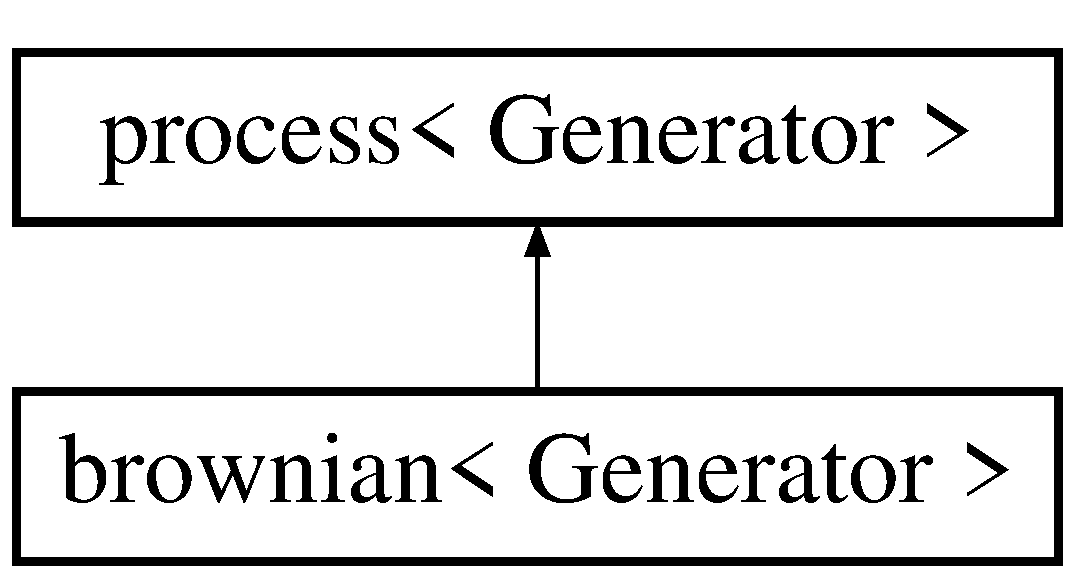
\includegraphics[height=2.000000cm]{classbrownian}
\end{center}
\end{figure}
\subsection*{Public Member Functions}
\begin{DoxyCompactItemize}
\item 
\mbox{\hyperlink{classbrownian_ab606472ba893b778b1ad3f57553354e3}{brownian}} ()
\begin{DoxyCompactList}\small\item\em Constructors \& destructors. \end{DoxyCompactList}\item 
\mbox{\Hypertarget{classbrownian_a11a807d65dafc80cadd54ab010db996a}\label{classbrownian_a11a807d65dafc80cadd54ab010db996a}} 
{\bfseries brownian} (double vol)
\item 
\mbox{\Hypertarget{classbrownian_afb58e5d64bc76193fcce54cf611f3671}\label{classbrownian_afb58e5d64bc76193fcce54cf611f3671}} 
std\+::vector$<$ double $>$ \mbox{\hyperlink{classbrownian_afb58e5d64bc76193fcce54cf611f3671}{next\+\_\+step}} (Generator \&gen, std\+::vector$<$ double $>$ state, double t)
\begin{DoxyCompactList}\small\item\em Next step. \end{DoxyCompactList}\end{DoxyCompactItemize}
\subsection*{Additional Inherited Members}


\subsection{Detailed Description}
\subsubsection*{template$<$typename Generator$>$\newline
class brownian$<$ Generator $>$}

A class to discretize a Brownian Motion with a classical Euler scheme. 

Mainly used for testing. 

\subsection{Constructor \& Destructor Documentation}
\mbox{\Hypertarget{classbrownian_ab606472ba893b778b1ad3f57553354e3}\label{classbrownian_ab606472ba893b778b1ad3f57553354e3}} 
\index{brownian@{brownian}!brownian@{brownian}}
\index{brownian@{brownian}!brownian@{brownian}}
\subsubsection{\texorpdfstring{brownian()}{brownian()}}
{\footnotesize\ttfamily template$<$typename Generator $>$ \\
\mbox{\hyperlink{classbrownian}{brownian}}$<$ Generator $>$\+::\mbox{\hyperlink{classbrownian}{brownian}} (\begin{DoxyParamCaption}{ }\end{DoxyParamCaption})}



Constructors \& destructors. 

Functions for the brownian class. 

The documentation for this class was generated from the following file\+:\begin{DoxyCompactItemize}
\item 
brownian.\+h\end{DoxyCompactItemize}

\hypertarget{classcir}{}\section{cir$<$ Generator $>$ Class Template Reference}
\label{classcir}\index{cir$<$ Generator $>$@{cir$<$ Generator $>$}}


Generation of a class with a C\+IR process.  




{\ttfamily \#include $<$cir.\+h$>$}

Inheritance diagram for cir$<$ Generator $>$\+:\begin{figure}[H]
\begin{center}
\leavevmode
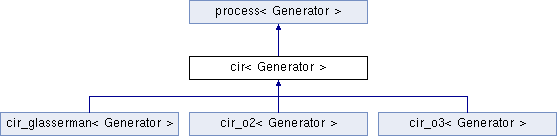
\includegraphics[height=2.994653cm]{classcir}
\end{center}
\end{figure}
\subsection*{Public Member Functions}
\begin{DoxyCompactItemize}
\item 
\mbox{\Hypertarget{classcir_af9a7a658975ddd029b12cd795ac04443}\label{classcir_af9a7a658975ddd029b12cd795ac04443}} 
\mbox{\hyperlink{classcir_af9a7a658975ddd029b12cd795ac04443}{cir}} ()
\begin{DoxyCompactList}\small\item\em Constructor. \end{DoxyCompactList}\item 
\mbox{\Hypertarget{classcir_adbb40f0d8743587d1ed5d2bb5728e315}\label{classcir_adbb40f0d8743587d1ed5d2bb5728e315}} 
\mbox{\hyperlink{classcir_adbb40f0d8743587d1ed5d2bb5728e315}{cir}} (double \mbox{\hyperlink{classprocess_ab4d01c8ea2e9c8285134786d32ae42aa}{state\+\_\+0}}, double \mbox{\hyperlink{classcir_aa5b05ff03ee8bb587ea94426a9ce704b}{k}}, double \mbox{\hyperlink{classcir_a358578305ea60d31c00546233304651c}{a}}, double s)
\begin{DoxyCompactList}\small\item\em Constructor. \end{DoxyCompactList}\item 
\mbox{\Hypertarget{classcir_a6b904f45a8f19eed507d814fbc09776f}\label{classcir_a6b904f45a8f19eed507d814fbc09776f}} 
\mbox{\hyperlink{classcir_a6b904f45a8f19eed507d814fbc09776f}{$\sim$cir}} ()
\begin{DoxyCompactList}\small\item\em Destructor. \end{DoxyCompactList}\item 
\mbox{\Hypertarget{classcir_ad3d4f7db1a4448632a6fdbada17cc651}\label{classcir_ad3d4f7db1a4448632a6fdbada17cc651}} 
virtual std\+::vector$<$ double $>$ \mbox{\hyperlink{classcir_ad3d4f7db1a4448632a6fdbada17cc651}{next\+\_\+step}} (Generator \&gen, std\+::vector$<$ double $>$ state, double t)=0
\begin{DoxyCompactList}\small\item\em Pure virtual function. Will be implemented in the different schemes. \end{DoxyCompactList}\item 
\mbox{\Hypertarget{classcir_a99e9faea04b897570b376e4495cdea53}\label{classcir_a99e9faea04b897570b376e4495cdea53}} 
double \mbox{\hyperlink{classcir_a99e9faea04b897570b376e4495cdea53}{get\+\_\+a}} ()
\begin{DoxyCompactList}\small\item\em Getter. \end{DoxyCompactList}\item 
\mbox{\Hypertarget{classcir_a3269ff6845cca07d9e99c139902fc3d4}\label{classcir_a3269ff6845cca07d9e99c139902fc3d4}} 
double \mbox{\hyperlink{classcir_a3269ff6845cca07d9e99c139902fc3d4}{get\+\_\+sigma}} ()
\begin{DoxyCompactList}\small\item\em Getter. \end{DoxyCompactList}\item 
\mbox{\Hypertarget{classcir_a071e1fa837b80e16de53f82223725bdf}\label{classcir_a071e1fa837b80e16de53f82223725bdf}} 
void \mbox{\hyperlink{classcir_a071e1fa837b80e16de53f82223725bdf}{set\+\_\+a}} (double \mbox{\hyperlink{classcir_a358578305ea60d31c00546233304651c}{a}})
\begin{DoxyCompactList}\small\item\em Setter. \end{DoxyCompactList}\item 
\mbox{\Hypertarget{classcir_a0f16e4b0fc9684e5ff41c7164bca2a2e}\label{classcir_a0f16e4b0fc9684e5ff41c7164bca2a2e}} 
void \mbox{\hyperlink{classcir_a0f16e4b0fc9684e5ff41c7164bca2a2e}{set\+\_\+sigma}} (double s)
\begin{DoxyCompactList}\small\item\em Setter. \end{DoxyCompactList}\end{DoxyCompactItemize}
\subsection*{Protected Attributes}
\begin{DoxyCompactItemize}
\item 
double \mbox{\hyperlink{classcir_a358578305ea60d31c00546233304651c}{a}}
\item 
double \mbox{\hyperlink{classcir_a76df757acc0179e1cdf766ed6627efc9}{sigma}}
\item 
double \mbox{\hyperlink{classcir_aa5b05ff03ee8bb587ea94426a9ce704b}{k}}
\end{DoxyCompactItemize}


\subsection{Detailed Description}
\subsubsection*{template$<$typename Generator$>$\newline
class cir$<$ Generator $>$}

Generation of a class with a C\+IR process. 

The class cir implements the class process. The C\+IR follows the dynamics dX = (a -\/ kX) dt + sigma sqrt(\+X) dW with X(0) = x\+\_\+0 

\subsection{Member Data Documentation}
\mbox{\Hypertarget{classcir_a358578305ea60d31c00546233304651c}\label{classcir_a358578305ea60d31c00546233304651c}} 
\index{cir@{cir}!a@{a}}
\index{a@{a}!cir@{cir}}
\subsubsection{\texorpdfstring{a}{a}}
{\footnotesize\ttfamily template$<$typename Generator $>$ \\
double \mbox{\hyperlink{classcir}{cir}}$<$ Generator $>$\+::a\hspace{0.3cm}{\ttfamily [protected]}}

Target value for C\+IR \mbox{\Hypertarget{classcir_aa5b05ff03ee8bb587ea94426a9ce704b}\label{classcir_aa5b05ff03ee8bb587ea94426a9ce704b}} 
\index{cir@{cir}!k@{k}}
\index{k@{k}!cir@{cir}}
\subsubsection{\texorpdfstring{k}{k}}
{\footnotesize\ttfamily template$<$typename Generator $>$ \\
double \mbox{\hyperlink{classcir}{cir}}$<$ Generator $>$\+::k\hspace{0.3cm}{\ttfamily [protected]}}

Mean reverting speed \mbox{\Hypertarget{classcir_a76df757acc0179e1cdf766ed6627efc9}\label{classcir_a76df757acc0179e1cdf766ed6627efc9}} 
\index{cir@{cir}!sigma@{sigma}}
\index{sigma@{sigma}!cir@{cir}}
\subsubsection{\texorpdfstring{sigma}{sigma}}
{\footnotesize\ttfamily template$<$typename Generator $>$ \\
double \mbox{\hyperlink{classcir}{cir}}$<$ Generator $>$\+::sigma\hspace{0.3cm}{\ttfamily [protected]}}

Volatility of volatility 

The documentation for this class was generated from the following file\+:\begin{DoxyCompactItemize}
\item 
cir.\+h\end{DoxyCompactItemize}

\hypertarget{classcir__glasserman}{}\section{cir\+\_\+glasserman$<$ Generator $>$ Class Template Reference}
\label{classcir__glasserman}\index{cir\+\_\+glasserman$<$ Generator $>$@{cir\+\_\+glasserman$<$ Generator $>$}}


An exact scheme for the C\+IR process.  




{\ttfamily \#include $<$cir.\+h$>$}



Inheritance diagram for cir\+\_\+glasserman$<$ Generator $>$\+:\nopagebreak
\begin{figure}[H]
\begin{center}
\leavevmode
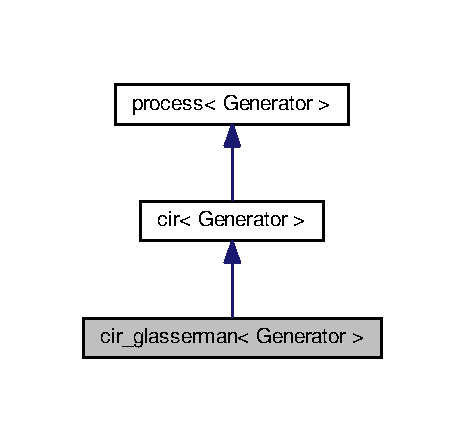
\includegraphics[width=223pt]{classcir__glasserman__inherit__graph}
\end{center}
\end{figure}


Collaboration diagram for cir\+\_\+glasserman$<$ Generator $>$\+:\nopagebreak
\begin{figure}[H]
\begin{center}
\leavevmode
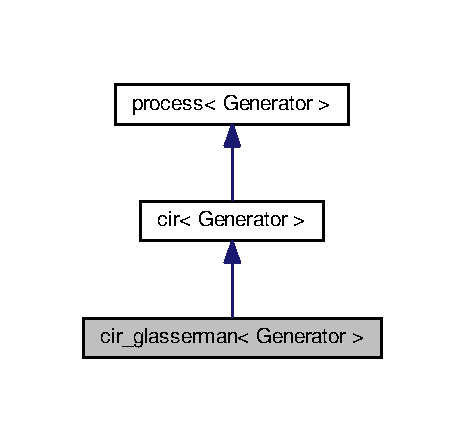
\includegraphics[width=223pt]{classcir__glasserman__coll__graph}
\end{center}
\end{figure}
\subsection*{Public Member Functions}
\begin{DoxyCompactItemize}
\item 
\hyperlink{classcir__glasserman_a992c04280cd4f2bca585df0e940cd928}{cir\+\_\+glasserman} ()\hypertarget{classcir__glasserman_a992c04280cd4f2bca585df0e940cd928}{}\label{classcir__glasserman_a992c04280cd4f2bca585df0e940cd928}

\begin{DoxyCompactList}\small\item\em Constructor. \end{DoxyCompactList}\item 
\hyperlink{classcir__glasserman_aa17f7ef0554ccd8a8e96779e9c8c501d}{cir\+\_\+glasserman} (double \hyperlink{classprocess_ab4d01c8ea2e9c8285134786d32ae42aa}{state\+\_\+0}, double \hyperlink{classcir_aa5b05ff03ee8bb587ea94426a9ce704b}{k}, double \hyperlink{classcir_a358578305ea60d31c00546233304651c}{a}, double s)\hypertarget{classcir__glasserman_aa17f7ef0554ccd8a8e96779e9c8c501d}{}\label{classcir__glasserman_aa17f7ef0554ccd8a8e96779e9c8c501d}

\begin{DoxyCompactList}\small\item\em Constructor. \end{DoxyCompactList}\item 
\hyperlink{classcir__glasserman_a75da65ee14fd95b6352e76a432144122}{$\sim$cir\+\_\+glasserman} ()\hypertarget{classcir__glasserman_a75da65ee14fd95b6352e76a432144122}{}\label{classcir__glasserman_a75da65ee14fd95b6352e76a432144122}

\begin{DoxyCompactList}\small\item\em Destructor. \end{DoxyCompactList}\item 
std\+::vector$<$ double $>$ \hyperlink{classcir__glasserman_aa3a48d9de6edccd4bfb8a52a5e5ad3df}{next\+\_\+step} (Generator \&gen, std\+::vector$<$ double $>$ state, double t)\hypertarget{classcir__glasserman_aa3a48d9de6edccd4bfb8a52a5e5ad3df}{}\label{classcir__glasserman_aa3a48d9de6edccd4bfb8a52a5e5ad3df}

\begin{DoxyCompactList}\small\item\em Pure virtual function. Will be implemented in the different schemes. \end{DoxyCompactList}\end{DoxyCompactItemize}
\subsection*{Protected Attributes}
\begin{DoxyCompactItemize}
\item 
std\+::poisson\+\_\+distribution$<$ int $>$ \hyperlink{classcir__glasserman_aed2bd8f09e275a2fd0012989771c61f7}{n\+\_\+poisson}
\begin{DoxyCompactList}\small\item\em Getters and Setters. \end{DoxyCompactList}\item 
std\+::chi\+\_\+squared\+\_\+distribution$<$ double $>$ \hyperlink{classcir__glasserman_a1f91410b367839c4b81e8e89e9597848}{x\+\_\+chi}
\item 
std\+::normal\+\_\+distribution$<$ double $>$ \hyperlink{classcir__glasserman_ab16c1db0bb521957833f67c690b6b8a4}{z\+\_\+norm}
\item 
double \hyperlink{classcir__glasserman_ad43d0610db68017bf054096cda60b27e}{d}
\end{DoxyCompactItemize}


\subsection{Detailed Description}
\subsubsection*{template$<$typename Generator$>$\\*
class cir\+\_\+glasserman$<$ Generator $>$}

An exact scheme for the C\+IR process. 

This class implements an exact scheme of discretization of the C\+IR process. It exploits the knowledge of the transition law of this process. It can be found in the book by Paul Glasserman. 

\subsection{Member Data Documentation}
\index{cir\+\_\+glasserman@{cir\+\_\+glasserman}!d@{d}}
\index{d@{d}!cir\+\_\+glasserman@{cir\+\_\+glasserman}}
\subsubsection[{\texorpdfstring{d}{d}}]{\setlength{\rightskip}{0pt plus 5cm}template$<$typename Generator $>$ double {\bf cir\+\_\+glasserman}$<$ Generator $>$\+::d\hspace{0.3cm}{\ttfamily [protected]}}\hypertarget{classcir__glasserman_ad43d0610db68017bf054096cda60b27e}{}\label{classcir__glasserman_ad43d0610db68017bf054096cda60b27e}
An auxiliary variable \index{cir\+\_\+glasserman@{cir\+\_\+glasserman}!n\+\_\+poisson@{n\+\_\+poisson}}
\index{n\+\_\+poisson@{n\+\_\+poisson}!cir\+\_\+glasserman@{cir\+\_\+glasserman}}
\subsubsection[{\texorpdfstring{n\+\_\+poisson}{n_poisson}}]{\setlength{\rightskip}{0pt plus 5cm}template$<$typename Generator $>$ std\+::poisson\+\_\+distribution$<$int$>$ {\bf cir\+\_\+glasserman}$<$ Generator $>$\+::n\+\_\+poisson\hspace{0.3cm}{\ttfamily [protected]}}\hypertarget{classcir__glasserman_aed2bd8f09e275a2fd0012989771c61f7}{}\label{classcir__glasserman_aed2bd8f09e275a2fd0012989771c61f7}


Getters and Setters. 

A Poisson random variable \index{cir\+\_\+glasserman@{cir\+\_\+glasserman}!x\+\_\+chi@{x\+\_\+chi}}
\index{x\+\_\+chi@{x\+\_\+chi}!cir\+\_\+glasserman@{cir\+\_\+glasserman}}
\subsubsection[{\texorpdfstring{x\+\_\+chi}{x_chi}}]{\setlength{\rightskip}{0pt plus 5cm}template$<$typename Generator $>$ std\+::chi\+\_\+squared\+\_\+distribution$<$double$>$ {\bf cir\+\_\+glasserman}$<$ Generator $>$\+::x\+\_\+chi\hspace{0.3cm}{\ttfamily [protected]}}\hypertarget{classcir__glasserman_a1f91410b367839c4b81e8e89e9597848}{}\label{classcir__glasserman_a1f91410b367839c4b81e8e89e9597848}
A Chi squared random variable \index{cir\+\_\+glasserman@{cir\+\_\+glasserman}!z\+\_\+norm@{z\+\_\+norm}}
\index{z\+\_\+norm@{z\+\_\+norm}!cir\+\_\+glasserman@{cir\+\_\+glasserman}}
\subsubsection[{\texorpdfstring{z\+\_\+norm}{z_norm}}]{\setlength{\rightskip}{0pt plus 5cm}template$<$typename Generator $>$ std\+::normal\+\_\+distribution$<$double$>$ {\bf cir\+\_\+glasserman}$<$ Generator $>$\+::z\+\_\+norm\hspace{0.3cm}{\ttfamily [protected]}}\hypertarget{classcir__glasserman_ab16c1db0bb521957833f67c690b6b8a4}{}\label{classcir__glasserman_ab16c1db0bb521957833f67c690b6b8a4}
A standard Normal random variable 

The documentation for this class was generated from the following file\+:\begin{DoxyCompactItemize}
\item 
/home/gregory/\+Desktop/\+Cours\+\_\+\+E\+K/\+P2/\+Pages\+\_\+projet/test\+\_\+git/proba\+\_\+num/src/cir.\+h\end{DoxyCompactItemize}

\hypertarget{classcir__o2}{}\section{cir\+\_\+o2$<$ Generator $>$ Class Template Reference}
\label{classcir__o2}\index{cir\+\_\+o2$<$ Generator $>$@{cir\+\_\+o2$<$ Generator $>$}}


A scheme of order 2 for the C\+IR process.  




{\ttfamily \#include $<$cir.\+h$>$}

Inheritance diagram for cir\+\_\+o2$<$ Generator $>$\+:\begin{figure}[H]
\begin{center}
\leavevmode
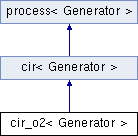
\includegraphics[height=3.000000cm]{classcir__o2}
\end{center}
\end{figure}
\subsection*{Public Member Functions}
\begin{DoxyCompactItemize}
\item 
\mbox{\Hypertarget{classcir__o2_a0f645b7ab87c6318ecb8f4654cef6ed7}\label{classcir__o2_a0f645b7ab87c6318ecb8f4654cef6ed7}} 
\mbox{\hyperlink{classcir__o2_a0f645b7ab87c6318ecb8f4654cef6ed7}{cir\+\_\+o2}} ()
\begin{DoxyCompactList}\small\item\em Constructor. \end{DoxyCompactList}\item 
\mbox{\Hypertarget{classcir__o2_ae29a2538f64d667ae2b5bbb4fa6a1964}\label{classcir__o2_ae29a2538f64d667ae2b5bbb4fa6a1964}} 
\mbox{\hyperlink{classcir__o2_ae29a2538f64d667ae2b5bbb4fa6a1964}{cir\+\_\+o2}} (double \mbox{\hyperlink{classprocess_ab4d01c8ea2e9c8285134786d32ae42aa}{state\+\_\+0}}, double \mbox{\hyperlink{classcir_aa5b05ff03ee8bb587ea94426a9ce704b}{k}}, double \mbox{\hyperlink{classcir_a358578305ea60d31c00546233304651c}{a}}, double s)
\begin{DoxyCompactList}\small\item\em Constructor. \end{DoxyCompactList}\item 
\mbox{\Hypertarget{classcir__o2_ac620cae85dd92526b320b885d33e1542}\label{classcir__o2_ac620cae85dd92526b320b885d33e1542}} 
\mbox{\hyperlink{classcir__o2_ac620cae85dd92526b320b885d33e1542}{$\sim$cir\+\_\+o2}} ()
\begin{DoxyCompactList}\small\item\em Destructor. \end{DoxyCompactList}\item 
\mbox{\Hypertarget{classcir__o2_aff77d63ff38cedf7f720f4bf081b3812}\label{classcir__o2_aff77d63ff38cedf7f720f4bf081b3812}} 
std\+::vector$<$ double $>$ \mbox{\hyperlink{classcir__o2_aff77d63ff38cedf7f720f4bf081b3812}{next\+\_\+step}} (Generator \&gen, std\+::vector$<$ double $>$ state, double t)
\begin{DoxyCompactList}\small\item\em Pure virtual function. Will be implemented in the different schemes. \end{DoxyCompactList}\end{DoxyCompactItemize}
\subsection*{Protected Attributes}
\begin{DoxyCompactItemize}
\item 
std\+::uniform\+\_\+real\+\_\+distribution$<$ double $>$ \mbox{\hyperlink{classcir__o2_a37d01ddf0963358ef44dcb20938b54fa}{u}}
\item 
\mbox{\hyperlink{classnormal__five__moments}{normal\+\_\+five\+\_\+moments}}$<$ Generator $>$ \mbox{\hyperlink{classcir__o2_a13719fb45e809812b9f62916d6baba2c}{y}}
\end{DoxyCompactItemize}


\subsection{Detailed Description}
\subsubsection*{template$<$typename Generator$>$\newline
class cir\+\_\+o2$<$ Generator $>$}

A scheme of order 2 for the C\+IR process. 

This class implements the Ninomiya-\/\+Victoir scheme for the C\+IR. It is of order 2. 

\subsection{Member Data Documentation}
\mbox{\Hypertarget{classcir__o2_a37d01ddf0963358ef44dcb20938b54fa}\label{classcir__o2_a37d01ddf0963358ef44dcb20938b54fa}} 
\index{cir\+\_\+o2@{cir\+\_\+o2}!u@{u}}
\index{u@{u}!cir\+\_\+o2@{cir\+\_\+o2}}
\subsubsection{\texorpdfstring{u}{u}}
{\footnotesize\ttfamily template$<$typename Generator $>$ \\
std\+::uniform\+\_\+real\+\_\+distribution$<$double$>$ \mbox{\hyperlink{classcir__o2}{cir\+\_\+o2}}$<$ Generator $>$\+::u\hspace{0.3cm}{\ttfamily [protected]}}

A uniform variable on \mbox{[}0,1\mbox{]} \mbox{\Hypertarget{classcir__o2_a13719fb45e809812b9f62916d6baba2c}\label{classcir__o2_a13719fb45e809812b9f62916d6baba2c}} 
\index{cir\+\_\+o2@{cir\+\_\+o2}!y@{y}}
\index{y@{y}!cir\+\_\+o2@{cir\+\_\+o2}}
\subsubsection{\texorpdfstring{y}{y}}
{\footnotesize\ttfamily template$<$typename Generator $>$ \\
\mbox{\hyperlink{classnormal__five__moments}{normal\+\_\+five\+\_\+moments}}$<$Generator$>$ \mbox{\hyperlink{classcir__o2}{cir\+\_\+o2}}$<$ Generator $>$\+::y\hspace{0.3cm}{\ttfamily [protected]}}

A random variable with the same first five moments as a standard Gaussian 

The documentation for this class was generated from the following file\+:\begin{DoxyCompactItemize}
\item 
cir.\+h\end{DoxyCompactItemize}

\hypertarget{classcir__o3}{}\section{cir\+\_\+o3$<$ Generator $>$ Class Template Reference}
\label{classcir__o3}\index{cir\+\_\+o3$<$ Generator $>$@{cir\+\_\+o3$<$ Generator $>$}}


A scheme of order 3 for the C\+IR process.  




{\ttfamily \#include $<$cir.\+h$>$}



Inheritance diagram for cir\+\_\+o3$<$ Generator $>$\+:\nopagebreak
\begin{figure}[H]
\begin{center}
\leavevmode
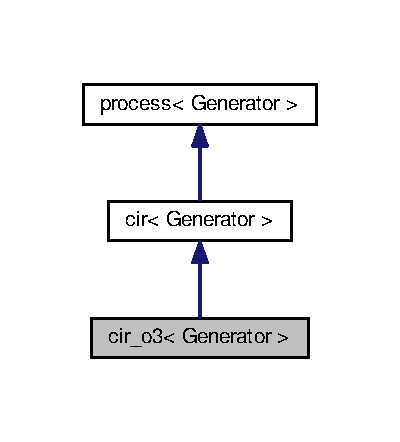
\includegraphics[width=192pt]{classcir__o3__inherit__graph}
\end{center}
\end{figure}


Collaboration diagram for cir\+\_\+o3$<$ Generator $>$\+:\nopagebreak
\begin{figure}[H]
\begin{center}
\leavevmode
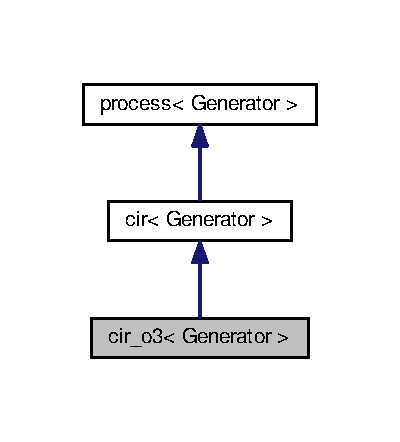
\includegraphics[width=192pt]{classcir__o3__coll__graph}
\end{center}
\end{figure}
\subsection*{Public Member Functions}
\begin{DoxyCompactItemize}
\item 
\hyperlink{classcir__o3_a73106636672bfd0236b2272e480a521c}{cir\+\_\+o3} ()\hypertarget{classcir__o3_a73106636672bfd0236b2272e480a521c}{}\label{classcir__o3_a73106636672bfd0236b2272e480a521c}

\begin{DoxyCompactList}\small\item\em Constructor. \end{DoxyCompactList}\item 
\hyperlink{classcir__o3_adda0ca25019f56ef8987af11c1b6a9ad}{cir\+\_\+o3} (double \hyperlink{classprocess_ab4d01c8ea2e9c8285134786d32ae42aa}{state\+\_\+0}, double \hyperlink{classcir_aa5b05ff03ee8bb587ea94426a9ce704b}{k}, double \hyperlink{classcir_a358578305ea60d31c00546233304651c}{a}, double s)\hypertarget{classcir__o3_adda0ca25019f56ef8987af11c1b6a9ad}{}\label{classcir__o3_adda0ca25019f56ef8987af11c1b6a9ad}

\begin{DoxyCompactList}\small\item\em Constructor. \end{DoxyCompactList}\item 
\hyperlink{classcir__o3_a8d51e7530a1170a835b548b601746537}{$\sim$cir\+\_\+o3} ()\hypertarget{classcir__o3_a8d51e7530a1170a835b548b601746537}{}\label{classcir__o3_a8d51e7530a1170a835b548b601746537}

\begin{DoxyCompactList}\small\item\em Destructor. \end{DoxyCompactList}\item 
std\+::vector$<$ double $>$ \hyperlink{classcir__o3_a77d0f79c0634f1d6cd19017e56eab451}{next\+\_\+step} (Generator \&gen, std\+::vector$<$ double $>$ state, double t)\hypertarget{classcir__o3_a77d0f79c0634f1d6cd19017e56eab451}{}\label{classcir__o3_a77d0f79c0634f1d6cd19017e56eab451}

\begin{DoxyCompactList}\small\item\em Pure virtual function. Will be implemented in the different schemes. \end{DoxyCompactList}\end{DoxyCompactItemize}
\subsection*{Protected Attributes}
\begin{DoxyCompactItemize}
\item 
std\+::uniform\+\_\+real\+\_\+distribution$<$ double $>$ \hyperlink{classcir__o3_a0e08c2c516a7f821a4a3ee8f9b0cf162}{u}
\item 
\hyperlink{classnormal__seven__moments}{normal\+\_\+seven\+\_\+moments}$<$ Generator $>$ \hyperlink{classcir__o3_a22d7ad16bc9bfb168095ab16ff0bc685}{seven}
\item 
\hyperlink{classzeta}{zeta}$<$ Generator $>$ \hyperlink{classcir__o3_aff6081fa06fbab8fd8bf06bbef2bf7c4}{zet}
\item 
\hyperlink{classrademacher}{rademacher}$<$ Generator $>$ \hyperlink{classcir__o3_a5ed2b331f33db9c48fde052e1a15a1d1}{rad}
\end{DoxyCompactItemize}


\subsection{Detailed Description}
\subsubsection*{template$<$typename Generator$>$\\*
class cir\+\_\+o3$<$ Generator $>$}

A scheme of order 3 for the C\+IR process. 

This class implements the Ninomiya-\/\+Victoir scheme for the C\+IR. It is of order 3. 

\subsection{Member Data Documentation}
\index{cir\+\_\+o3@{cir\+\_\+o3}!rad@{rad}}
\index{rad@{rad}!cir\+\_\+o3@{cir\+\_\+o3}}
\subsubsection[{\texorpdfstring{rad}{rad}}]{\setlength{\rightskip}{0pt plus 5cm}template$<$typename Generator $>$ {\bf rademacher}$<$Generator$>$ {\bf cir\+\_\+o3}$<$ Generator $>$\+::rad\hspace{0.3cm}{\ttfamily [protected]}}\hypertarget{classcir__o3_a5ed2b331f33db9c48fde052e1a15a1d1}{}\label{classcir__o3_a5ed2b331f33db9c48fde052e1a15a1d1}
A Rademacher random variable \index{cir\+\_\+o3@{cir\+\_\+o3}!seven@{seven}}
\index{seven@{seven}!cir\+\_\+o3@{cir\+\_\+o3}}
\subsubsection[{\texorpdfstring{seven}{seven}}]{\setlength{\rightskip}{0pt plus 5cm}template$<$typename Generator $>$ {\bf normal\+\_\+seven\+\_\+moments}$<$Generator$>$ {\bf cir\+\_\+o3}$<$ Generator $>$\+::seven\hspace{0.3cm}{\ttfamily [protected]}}\hypertarget{classcir__o3_a22d7ad16bc9bfb168095ab16ff0bc685}{}\label{classcir__o3_a22d7ad16bc9bfb168095ab16ff0bc685}
A random variable with the same first seven moments as a standard Gaussian \index{cir\+\_\+o3@{cir\+\_\+o3}!u@{u}}
\index{u@{u}!cir\+\_\+o3@{cir\+\_\+o3}}
\subsubsection[{\texorpdfstring{u}{u}}]{\setlength{\rightskip}{0pt plus 5cm}template$<$typename Generator $>$ std\+::uniform\+\_\+real\+\_\+distribution$<$double$>$ {\bf cir\+\_\+o3}$<$ Generator $>$\+::u\hspace{0.3cm}{\ttfamily [protected]}}\hypertarget{classcir__o3_a0e08c2c516a7f821a4a3ee8f9b0cf162}{}\label{classcir__o3_a0e08c2c516a7f821a4a3ee8f9b0cf162}
A uniform variable on \mbox{[}0,1\mbox{]} \index{cir\+\_\+o3@{cir\+\_\+o3}!zet@{zet}}
\index{zet@{zet}!cir\+\_\+o3@{cir\+\_\+o3}}
\subsubsection[{\texorpdfstring{zet}{zet}}]{\setlength{\rightskip}{0pt plus 5cm}template$<$typename Generator $>$ {\bf zeta}$<$Generator$>$ {\bf cir\+\_\+o3}$<$ Generator $>$\+::zet\hspace{0.3cm}{\ttfamily [protected]}}\hypertarget{classcir__o3_aff6081fa06fbab8fd8bf06bbef2bf7c4}{}\label{classcir__o3_aff6081fa06fbab8fd8bf06bbef2bf7c4}
A uniform variable on \{1,2,3\} 

The documentation for this class was generated from the following file\+:\begin{DoxyCompactItemize}
\item 
/home/gregory/\+Desktop/\+Cours\+\_\+\+E\+K/\+P2/\+Pages\+\_\+projet/test\+\_\+git/proba\+\_\+num/src/cir.\+h\end{DoxyCompactItemize}

\hypertarget{classheston}{}\section{heston$<$ Generator, Cir $>$ Class Template Reference}
\label{classheston}\index{heston$<$ Generator, Cir $>$@{heston$<$ Generator, Cir $>$}}


Generation of a class with a Heston process.  




{\ttfamily \#include $<$heston.\+h$>$}



Inheritance diagram for heston$<$ Generator, Cir $>$\+:\nopagebreak
\begin{figure}[H]
\begin{center}
\leavevmode
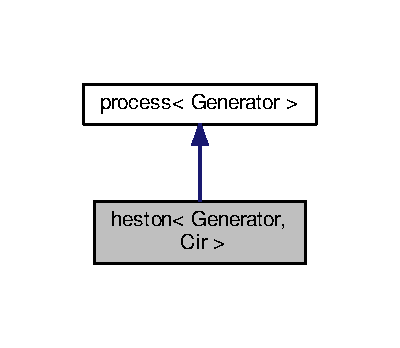
\includegraphics[width=192pt]{classheston__inherit__graph}
\end{center}
\end{figure}


Collaboration diagram for heston$<$ Generator, Cir $>$\+:\nopagebreak
\begin{figure}[H]
\begin{center}
\leavevmode
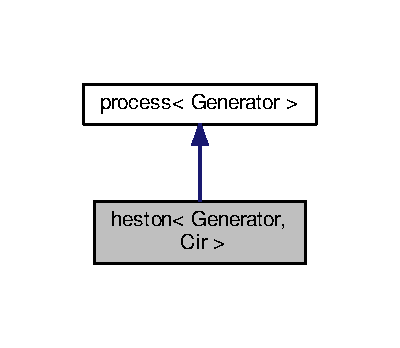
\includegraphics[width=192pt]{classheston__coll__graph}
\end{center}
\end{figure}
\subsection*{Public Member Functions}
\begin{DoxyCompactItemize}
\item 
\hyperlink{classheston_a3938ade2d7a6d3af9130bba2066618d2}{heston} ()\hypertarget{classheston_a3938ade2d7a6d3af9130bba2066618d2}{}\label{classheston_a3938ade2d7a6d3af9130bba2066618d2}

\begin{DoxyCompactList}\small\item\em Constructor. \end{DoxyCompactList}\item 
\hyperlink{classheston_a443a0ec8ea9e1c14576f7ba6ca602dd4}{$\sim$heston} ()\hypertarget{classheston_a443a0ec8ea9e1c14576f7ba6ca602dd4}{}\label{classheston_a443a0ec8ea9e1c14576f7ba6ca602dd4}

\begin{DoxyCompactList}\small\item\em Destructor. \end{DoxyCompactList}\item 
\hyperlink{classheston_a377c1e6ea58b4078f1ae4ddef05d7251}{heston} (double cir\+\_\+0, double x\+\_\+0, double a, double k, double sigma, double rho, double r)\hypertarget{classheston_a377c1e6ea58b4078f1ae4ddef05d7251}{}\label{classheston_a377c1e6ea58b4078f1ae4ddef05d7251}

\begin{DoxyCompactList}\small\item\em Constructor. \end{DoxyCompactList}\item 
std\+::vector$<$ double $>$ {\bfseries hw} (Generator \&gen, std\+::vector$<$ double $>$ state, double t)\hypertarget{classheston_ae71c07c92e43ecf8320baa4085fc67b1}{}\label{classheston_ae71c07c92e43ecf8320baa4085fc67b1}

\item 
std\+::vector$<$ double $>$ {\bfseries hz} (Generator \&gen, std\+::vector$<$ double $>$ state, double t)\hypertarget{classheston_a901689fa5b94062ec3b1b1371d0107fa}{}\label{classheston_a901689fa5b94062ec3b1b1371d0107fa}

\item 
std\+::vector$<$ double $>$ \hyperlink{classheston_a81ef826578f2a62320698e88cc2b1b3b}{next\+\_\+step} (Generator \&gen, std\+::vector$<$ double $>$ state, double t)
\begin{DoxyCompactList}\small\item\em Function Next Step. \end{DoxyCompactList}\item 
double \hyperlink{classheston_a574fdb0c7e744e931bf3e8fd000ea5ca}{log\+\_\+spot\+\_\+one} (double t)
\end{DoxyCompactItemize}
\subsection*{Additional Inherited Members}


\subsection{Detailed Description}
\subsubsection*{template$<$typename Generator, typename Cir$>$\\*
class heston$<$ Generator, Cir $>$}

Generation of a class with a Heston process. 

The class heston implements the class process. We compute the classical Heston model, along with the integrals of the price and the vol. 

\subsection{Member Function Documentation}
\index{heston@{heston}!log\+\_\+spot\+\_\+one@{log\+\_\+spot\+\_\+one}}
\index{log\+\_\+spot\+\_\+one@{log\+\_\+spot\+\_\+one}!heston@{heston}}
\subsubsection[{\texorpdfstring{log\+\_\+spot\+\_\+one(double t)}{log_spot_one(double t)}}]{\setlength{\rightskip}{0pt plus 5cm}template$<$typename Generator , typename Cir $>$ double {\bf heston}$<$ Generator, Cir $>$\+::log\+\_\+spot\+\_\+one (
\begin{DoxyParamCaption}
\item[{double}]{t}
\end{DoxyParamCaption}
)}\hypertarget{classheston_a574fdb0c7e744e931bf3e8fd000ea5ca}{}\label{classheston_a574fdb0c7e744e931bf3e8fd000ea5ca}
Computes the exact mean of log(\+S\+\_\+t) where S is the price process. Useful for variance reduction by a control variate technique. \index{heston@{heston}!next\+\_\+step@{next\+\_\+step}}
\index{next\+\_\+step@{next\+\_\+step}!heston@{heston}}
\subsubsection[{\texorpdfstring{next\+\_\+step(\+Generator \&gen, std\+::vector$<$ double $>$ state, double t)}{next_step(Generator &gen, std::vector< double > state, double t)}}]{\setlength{\rightskip}{0pt plus 5cm}template$<$typename Generator , typename Cir $>$ std\+::vector$<$ double $>$ {\bf heston}$<$ Generator, Cir $>$\+::next\+\_\+step (
\begin{DoxyParamCaption}
\item[{Generator \&}]{gen, }
\item[{std\+::vector$<$ double $>$}]{state, }
\item[{double}]{t}
\end{DoxyParamCaption}
)\hspace{0.3cm}{\ttfamily [virtual]}}\hypertarget{classheston_a81ef826578f2a62320698e88cc2b1b3b}{}\label{classheston_a81ef826578f2a62320698e88cc2b1b3b}


Function Next Step. 

Pure virtual function that will be over-\/written for every instance of process. Computes the value of the discretized process at time t + time\+\_\+step. The value of the discretized process at t is stored in state. 

Implements \hyperlink{classprocess_a55c46e4b4ab1992ce09f4133fb484fd6}{process$<$ Generator $>$}.



The documentation for this class was generated from the following file\+:\begin{DoxyCompactItemize}
\item 
/home/gregory/\+Desktop/\+Cours\+\_\+\+E\+K/\+P2/\+Pages\+\_\+projet/test\+\_\+git/proba\+\_\+num/src/heston.\+h\end{DoxyCompactItemize}

\hypertarget{classintegral__brownian}{}\section{integral\+\_\+brownian$<$ Generator $>$ Class Template Reference}
\label{classintegral__brownian}\index{integral\+\_\+brownian$<$ Generator $>$@{integral\+\_\+brownian$<$ Generator $>$}}


A class to simulate the integral of a Brownian Motion with a classical Euler scheme.  




{\ttfamily \#include $<$integral\+\_\+brownian.\+h$>$}



Inheritance diagram for integral\+\_\+brownian$<$ Generator $>$\+:\nopagebreak
\begin{figure}[H]
\begin{center}
\leavevmode
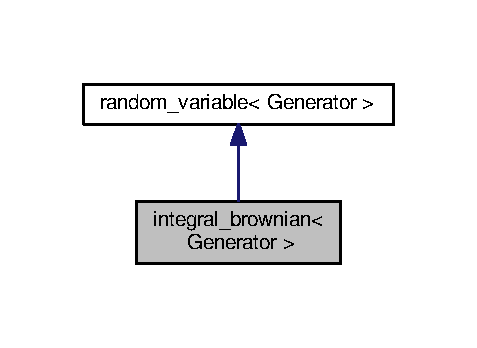
\includegraphics[width=229pt]{classintegral__brownian__inherit__graph}
\end{center}
\end{figure}


Collaboration diagram for integral\+\_\+brownian$<$ Generator $>$\+:\nopagebreak
\begin{figure}[H]
\begin{center}
\leavevmode
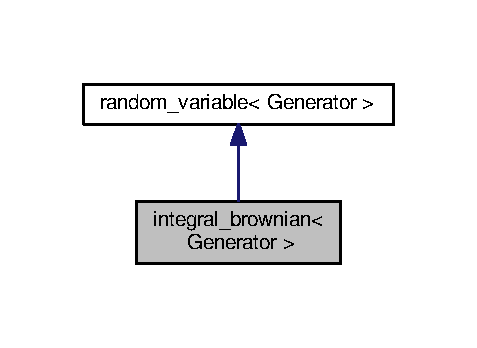
\includegraphics[width=229pt]{classintegral__brownian__coll__graph}
\end{center}
\end{figure}
\subsection*{Public Member Functions}
\begin{DoxyCompactItemize}
\item 
{\bfseries integral\+\_\+brownian} (unsigned int number\+\_\+steps)\hypertarget{classintegral__brownian_acbb676c9fb27ebd1de72f9dda5e2bbbf}{}\label{classintegral__brownian_acbb676c9fb27ebd1de72f9dda5e2bbbf}

\item 
double \hyperlink{classintegral__brownian_a974ec7d678079bc1acdc691a506a3092}{operator()} (Generator \&gen)\hypertarget{classintegral__brownian_a974ec7d678079bc1acdc691a506a3092}{}\label{classintegral__brownian_a974ec7d678079bc1acdc691a506a3092}

\begin{DoxyCompactList}\small\item\em Virtual function. \end{DoxyCompactList}\end{DoxyCompactItemize}
\subsection*{Additional Inherited Members}


\subsection{Detailed Description}
\subsubsection*{template$<$typename Generator$>$\\*
class integral\+\_\+brownian$<$ Generator $>$}

A class to simulate the integral of a Brownian Motion with a classical Euler scheme. 

Mainly used for testing. 

The documentation for this class was generated from the following file\+:\begin{DoxyCompactItemize}
\item 
/home/gregory/\+Desktop/\+Cours\+\_\+\+E\+K/\+P2/\+Pages\+\_\+projet/test\+\_\+git/proba\+\_\+num/src/integral\+\_\+brownian.\+h\end{DoxyCompactItemize}

\hypertarget{classmonte__carlo}{}\section{monte\+\_\+carlo$<$ Generator $>$ Class Template Reference}
\label{classmonte__carlo}\index{monte\+\_\+carlo$<$ Generator $>$@{monte\+\_\+carlo$<$ Generator $>$}}


A general class for Monte-\/\+Carlo simulation.  




{\ttfamily \#include $<$monte\+\_\+carlo.\+h$>$}

\subsection*{Public Member Functions}
\begin{DoxyCompactItemize}
\item 
\mbox{\hyperlink{classmonte__carlo_a602098d8c4cd2400e8b6036a7526437d}{monte\+\_\+carlo}} ()
\begin{DoxyCompactList}\small\item\em Constructors \& destructors. \end{DoxyCompactList}\item 
\mbox{\hyperlink{classmonte__carlo_a3c7619083f106006f7549bfa21af0b70}{monte\+\_\+carlo}} (\mbox{\hyperlink{classrandom__variable}{random\+\_\+variable}}$<$ Generator $>$ $\ast$rv)
\item 
\mbox{\Hypertarget{classmonte__carlo_ae8ba9ec39bb65da0a1d4c5881c3c57d9}\label{classmonte__carlo_ae8ba9ec39bb65da0a1d4c5881c3c57d9}} 
double \mbox{\hyperlink{classmonte__carlo_ae8ba9ec39bb65da0a1d4c5881c3c57d9}{get\+\_\+precision}} ()
\begin{DoxyCompactList}\small\item\em Getter. \end{DoxyCompactList}\item 
\mbox{\Hypertarget{classmonte__carlo_af73122a99655bfdd93d5b72f32ea8ff1}\label{classmonte__carlo_af73122a99655bfdd93d5b72f32ea8ff1}} 
unsigned int \mbox{\hyperlink{classmonte__carlo_af73122a99655bfdd93d5b72f32ea8ff1}{get\+\_\+cap}} ()
\begin{DoxyCompactList}\small\item\em Getter. \end{DoxyCompactList}\item 
\mbox{\Hypertarget{classmonte__carlo_af771b7b89e0ff85acfff8d6156a35cbf}\label{classmonte__carlo_af771b7b89e0ff85acfff8d6156a35cbf}} 
double \mbox{\hyperlink{classmonte__carlo_af771b7b89e0ff85acfff8d6156a35cbf}{get\+\_\+mean}} ()
\begin{DoxyCompactList}\small\item\em Getter. \end{DoxyCompactList}\item 
\mbox{\Hypertarget{classmonte__carlo_afff42d06090878c287928c375e9713d2}\label{classmonte__carlo_afff42d06090878c287928c375e9713d2}} 
double \mbox{\hyperlink{classmonte__carlo_afff42d06090878c287928c375e9713d2}{get\+\_\+std}} ()
\begin{DoxyCompactList}\small\item\em Getter. \end{DoxyCompactList}\item 
\mbox{\Hypertarget{classmonte__carlo_a1e83d23fdb90bc2680a2820151250c6f}\label{classmonte__carlo_a1e83d23fdb90bc2680a2820151250c6f}} 
std\+::pair$<$ double, double $>$ \mbox{\hyperlink{classmonte__carlo_a1e83d23fdb90bc2680a2820151250c6f}{get\+\_\+confidence\+\_\+interval}} ()
\begin{DoxyCompactList}\small\item\em Getter. \end{DoxyCompactList}\item 
\mbox{\Hypertarget{classmonte__carlo_a4630da58a98e8f080c124b6be1239849}\label{classmonte__carlo_a4630da58a98e8f080c124b6be1239849}} 
void \mbox{\hyperlink{classmonte__carlo_a4630da58a98e8f080c124b6be1239849}{set\+\_\+precision}} (double p)
\begin{DoxyCompactList}\small\item\em Setter. \end{DoxyCompactList}\item 
\mbox{\Hypertarget{classmonte__carlo_aa73333519c4f888338def6b93a125304}\label{classmonte__carlo_aa73333519c4f888338def6b93a125304}} 
void \mbox{\hyperlink{classmonte__carlo_aa73333519c4f888338def6b93a125304}{set\+\_\+cap}} (unsigned int c)
\begin{DoxyCompactList}\small\item\em Setter. \end{DoxyCompactList}\item 
\mbox{\Hypertarget{classmonte__carlo_ad4dbf4b40cadbacc3beadd7fd3721d0b}\label{classmonte__carlo_ad4dbf4b40cadbacc3beadd7fd3721d0b}} 
double \mbox{\hyperlink{classmonte__carlo_ad4dbf4b40cadbacc3beadd7fd3721d0b}{simulate}} (Generator \&gen)
\begin{DoxyCompactList}\small\item\em Simulation of one realisation of the random variable. \end{DoxyCompactList}\item 
void \mbox{\hyperlink{classmonte__carlo_a598c1fbac6b56ee278fd04bf6115b1d3}{compute}} (Generator \&gen)
\begin{DoxyCompactList}\small\item\em Computations of a naive Monte Carlo estimator. \end{DoxyCompactList}\item 
void \mbox{\hyperlink{classmonte__carlo_a5fb1de57e0f77deb8ff167589b9e8b9e}{print}} ()
\begin{DoxyCompactList}\small\item\em Printing the results. \end{DoxyCompactList}\end{DoxyCompactItemize}
\subsection*{Public Attributes}
\begin{DoxyCompactItemize}
\item 
\mbox{\Hypertarget{classmonte__carlo_ad179708fe615012fcaa71adfb013cf3b}\label{classmonte__carlo_ad179708fe615012fcaa71adfb013cf3b}} 
\mbox{\hyperlink{classrandom__variable}{random\+\_\+variable}}$<$ Generator $>$ $\ast$ {\bfseries variable}
\item 
\mbox{\Hypertarget{classmonte__carlo_a62d218e17216c5cd8db237d2e446f950}\label{classmonte__carlo_a62d218e17216c5cd8db237d2e446f950}} 
bool {\bfseries computed}
\item 
\mbox{\Hypertarget{classmonte__carlo_a7ef35469245e3f4d91c822ece547aa66}\label{classmonte__carlo_a7ef35469245e3f4d91c822ece547aa66}} 
bool {\bfseries successful}
\item 
\mbox{\Hypertarget{classmonte__carlo_a27a554ebe8e1847fee8291ed93f24423}\label{classmonte__carlo_a27a554ebe8e1847fee8291ed93f24423}} 
double {\bfseries precision}
\item 
\mbox{\Hypertarget{classmonte__carlo_ac0f656225be3c3d9bf7eb0edfa4e95c6}\label{classmonte__carlo_ac0f656225be3c3d9bf7eb0edfa4e95c6}} 
unsigned int {\bfseries cap\+\_\+iterations}
\item 
\mbox{\Hypertarget{classmonte__carlo_ade5ed60cafd32398a80daf71859a824e}\label{classmonte__carlo_ade5ed60cafd32398a80daf71859a824e}} 
unsigned int {\bfseries count}
\item 
\mbox{\Hypertarget{classmonte__carlo_aedf0cabb9a89b2b02aa63dc8b00e34d5}\label{classmonte__carlo_aedf0cabb9a89b2b02aa63dc8b00e34d5}} 
double {\bfseries empirical\+\_\+mean}
\item 
\mbox{\Hypertarget{classmonte__carlo_af698280f1f16c333b108f06e41b45c7e}\label{classmonte__carlo_af698280f1f16c333b108f06e41b45c7e}} 
double {\bfseries empirical\+\_\+var}
\item 
\mbox{\Hypertarget{classmonte__carlo_a22d78794a12eabe859d6249b7206aa6a}\label{classmonte__carlo_a22d78794a12eabe859d6249b7206aa6a}} 
double {\bfseries empirical\+\_\+std}
\item 
\mbox{\Hypertarget{classmonte__carlo_ad02f29a48b9977ff00ec9044bfde2f03}\label{classmonte__carlo_ad02f29a48b9977ff00ec9044bfde2f03}} 
double {\bfseries ci\+\_\+l\+\_\+bound}
\item 
\mbox{\Hypertarget{classmonte__carlo_a2c0e5849e8a88c643706159019b24476}\label{classmonte__carlo_a2c0e5849e8a88c643706159019b24476}} 
double {\bfseries ci\+\_\+h\+\_\+bound}
\end{DoxyCompactItemize}


\subsection{Detailed Description}
\subsubsection*{template$<$typename Generator$>$\newline
class monte\+\_\+carlo$<$ Generator $>$}

A general class for Monte-\/\+Carlo simulation. 

In this class we compute naive MC estimators (with confidence interval) given a random variable. We also implement different variance reduction techniques. 

\subsection{Constructor \& Destructor Documentation}
\mbox{\Hypertarget{classmonte__carlo_a602098d8c4cd2400e8b6036a7526437d}\label{classmonte__carlo_a602098d8c4cd2400e8b6036a7526437d}} 
\index{monte\+\_\+carlo@{monte\+\_\+carlo}!monte\+\_\+carlo@{monte\+\_\+carlo}}
\index{monte\+\_\+carlo@{monte\+\_\+carlo}!monte\+\_\+carlo@{monte\+\_\+carlo}}
\subsubsection{\texorpdfstring{monte\+\_\+carlo()}{monte\_carlo()}\hspace{0.1cm}{\footnotesize\ttfamily [1/2]}}
{\footnotesize\ttfamily template$<$typename Generator $>$ \\
\mbox{\hyperlink{classmonte__carlo}{monte\+\_\+carlo}}$<$ Generator $>$\+::\mbox{\hyperlink{classmonte__carlo}{monte\+\_\+carlo}} (\begin{DoxyParamCaption}{ }\end{DoxyParamCaption})}



Constructors \& destructors. 

All this are default values

By default, the variable we integrate is a N(0, 1) \mbox{\Hypertarget{classmonte__carlo_a3c7619083f106006f7549bfa21af0b70}\label{classmonte__carlo_a3c7619083f106006f7549bfa21af0b70}} 
\index{monte\+\_\+carlo@{monte\+\_\+carlo}!monte\+\_\+carlo@{monte\+\_\+carlo}}
\index{monte\+\_\+carlo@{monte\+\_\+carlo}!monte\+\_\+carlo@{monte\+\_\+carlo}}
\subsubsection{\texorpdfstring{monte\+\_\+carlo()}{monte\_carlo()}\hspace{0.1cm}{\footnotesize\ttfamily [2/2]}}
{\footnotesize\ttfamily template$<$typename Generator $>$ \\
\mbox{\hyperlink{classmonte__carlo}{monte\+\_\+carlo}}$<$ Generator $>$\+::\mbox{\hyperlink{classmonte__carlo}{monte\+\_\+carlo}} (\begin{DoxyParamCaption}\item[{\mbox{\hyperlink{classrandom__variable}{random\+\_\+variable}}$<$ Generator $>$ $\ast$}]{rv }\end{DoxyParamCaption})}

The random variable we want to integrate

All these are default values. 

\subsection{Member Function Documentation}
\mbox{\Hypertarget{classmonte__carlo_a598c1fbac6b56ee278fd04bf6115b1d3}\label{classmonte__carlo_a598c1fbac6b56ee278fd04bf6115b1d3}} 
\index{monte\+\_\+carlo@{monte\+\_\+carlo}!compute@{compute}}
\index{compute@{compute}!monte\+\_\+carlo@{monte\+\_\+carlo}}
\subsubsection{\texorpdfstring{compute()}{compute()}}
{\footnotesize\ttfamily template$<$typename Generator $>$ \\
void \mbox{\hyperlink{classmonte__carlo}{monte\+\_\+carlo}}$<$ Generator $>$\+::compute (\begin{DoxyParamCaption}\item[{Generator \&}]{gen }\end{DoxyParamCaption})}



Computations of a naive Monte Carlo estimator. 

This is the method that computes a naive MC estimator \mbox{\Hypertarget{classmonte__carlo_a5fb1de57e0f77deb8ff167589b9e8b9e}\label{classmonte__carlo_a5fb1de57e0f77deb8ff167589b9e8b9e}} 
\index{monte\+\_\+carlo@{monte\+\_\+carlo}!print@{print}}
\index{print@{print}!monte\+\_\+carlo@{monte\+\_\+carlo}}
\subsubsection{\texorpdfstring{print()}{print()}}
{\footnotesize\ttfamily template$<$typename Generator $>$ \\
void \mbox{\hyperlink{classmonte__carlo}{monte\+\_\+carlo}}$<$ Generator $>$\+::print (\begin{DoxyParamCaption}{ }\end{DoxyParamCaption})}



Printing the results. 

Printing our results properly 

The documentation for this class was generated from the following file\+:\begin{DoxyCompactItemize}
\item 
monte\+\_\+carlo.\+h\end{DoxyCompactItemize}

\hypertarget{classnormal}{}\section{normal$<$ Generator $>$ Class Template Reference}
\label{classnormal}\index{normal$<$ Generator $>$@{normal$<$ Generator $>$}}


A class to simulate a normal random variable.  




{\ttfamily \#include $<$normal.\+h$>$}



Inheritance diagram for normal$<$ Generator $>$\+:\nopagebreak
\begin{figure}[H]
\begin{center}
\leavevmode
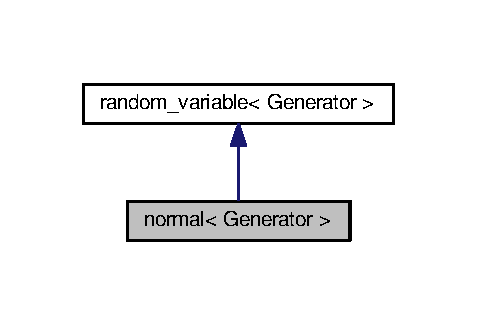
\includegraphics[width=229pt]{classnormal__inherit__graph}
\end{center}
\end{figure}


Collaboration diagram for normal$<$ Generator $>$\+:\nopagebreak
\begin{figure}[H]
\begin{center}
\leavevmode
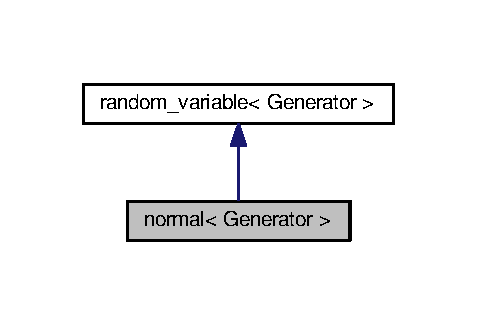
\includegraphics[width=229pt]{classnormal__coll__graph}
\end{center}
\end{figure}
\subsection*{Public Member Functions}
\begin{DoxyCompactItemize}
\item 
{\bfseries normal} (double m, double s)\hypertarget{classnormal_af8582789d606124cf4cfdf981c7b5943}{}\label{classnormal_af8582789d606124cf4cfdf981c7b5943}

\item 
double \hyperlink{classnormal_a56c48e011ff2fbce46aea55f1efbbbc1}{operator()} (Generator \&gen)\hypertarget{classnormal_a56c48e011ff2fbce46aea55f1efbbbc1}{}\label{classnormal_a56c48e011ff2fbce46aea55f1efbbbc1}

\begin{DoxyCompactList}\small\item\em Virtual function. \end{DoxyCompactList}\end{DoxyCompactItemize}
\subsection*{Additional Inherited Members}


\subsection{Detailed Description}
\subsubsection*{template$<$typename Generator$>$\\*
class normal$<$ Generator $>$}

A class to simulate a normal random variable. 

The documentation for this class was generated from the following file\+:\begin{DoxyCompactItemize}
\item 
/home/gregory/\+Desktop/\+Cours\+\_\+\+E\+K/\+P2/\+Pages\+\_\+projet/test\+\_\+git/proba\+\_\+num/src/normal.\+h\end{DoxyCompactItemize}

\hypertarget{classnormal__five__moments}{}\section{normal\+\_\+five\+\_\+moments$<$ Generator $>$ Class Template Reference}
\label{classnormal__five__moments}\index{normal\+\_\+five\+\_\+moments$<$ Generator $>$@{normal\+\_\+five\+\_\+moments$<$ Generator $>$}}


A class to simulate a random variable with the same first five moments as a standard Gaussian.  




{\ttfamily \#include $<$normal.\+h$>$}



Inheritance diagram for normal\+\_\+five\+\_\+moments$<$ Generator $>$\+:\nopagebreak
\begin{figure}[H]
\begin{center}
\leavevmode
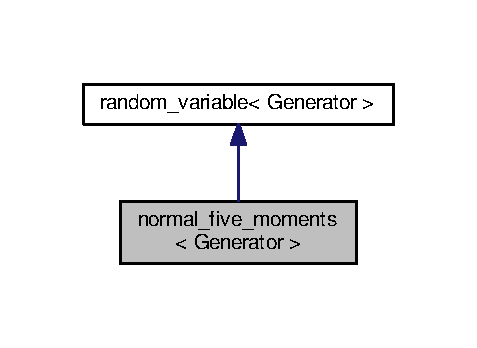
\includegraphics[width=229pt]{classnormal__five__moments__inherit__graph}
\end{center}
\end{figure}


Collaboration diagram for normal\+\_\+five\+\_\+moments$<$ Generator $>$\+:\nopagebreak
\begin{figure}[H]
\begin{center}
\leavevmode
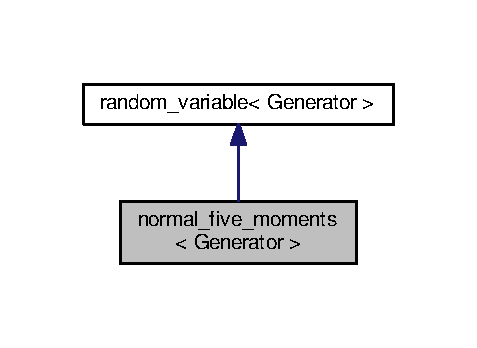
\includegraphics[width=229pt]{classnormal__five__moments__coll__graph}
\end{center}
\end{figure}
\subsection*{Public Member Functions}
\begin{DoxyCompactItemize}
\item 
double \hyperlink{classnormal__five__moments_adca4add1bfd8ea199bd63c80ab48b2d1}{operator()} (Generator \&gen)\hypertarget{classnormal__five__moments_adca4add1bfd8ea199bd63c80ab48b2d1}{}\label{classnormal__five__moments_adca4add1bfd8ea199bd63c80ab48b2d1}

\begin{DoxyCompactList}\small\item\em Virtual function. \end{DoxyCompactList}\end{DoxyCompactItemize}
\subsection*{Additional Inherited Members}


\subsection{Detailed Description}
\subsubsection*{template$<$typename Generator$>$\\*
class normal\+\_\+five\+\_\+moments$<$ Generator $>$}

A class to simulate a random variable with the same first five moments as a standard Gaussian. 

The documentation for this class was generated from the following file\+:\begin{DoxyCompactItemize}
\item 
/home/gregory/\+Desktop/\+Cours\+\_\+\+E\+K/\+P2/\+Pages\+\_\+projet/test\+\_\+git/proba\+\_\+num/src/normal.\+h\end{DoxyCompactItemize}

\hypertarget{classnormal__seven__moments}{}\section{normal\+\_\+seven\+\_\+moments$<$ Generator $>$ Class Template Reference}
\label{classnormal__seven__moments}\index{normal\+\_\+seven\+\_\+moments$<$ Generator $>$@{normal\+\_\+seven\+\_\+moments$<$ Generator $>$}}


A class to simulate a random variable with the same first seven moments as a standard Gaussian.  




{\ttfamily \#include $<$normal.\+h$>$}

Inheritance diagram for normal\+\_\+seven\+\_\+moments$<$ Generator $>$\+:\begin{figure}[H]
\begin{center}
\leavevmode
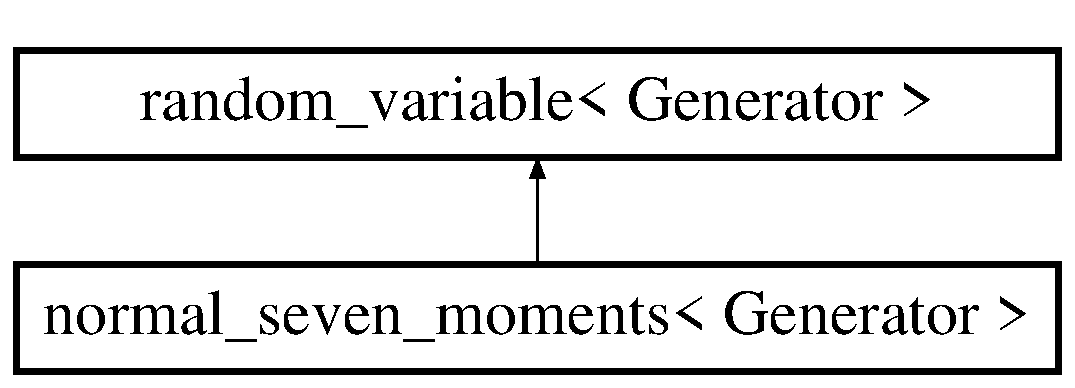
\includegraphics[height=2.000000cm]{classnormal__seven__moments}
\end{center}
\end{figure}
\subsection*{Public Member Functions}
\begin{DoxyCompactItemize}
\item 
\mbox{\Hypertarget{classnormal__seven__moments_a45d2d30b82cd449a4e3e2d9fe266b786}\label{classnormal__seven__moments_a45d2d30b82cd449a4e3e2d9fe266b786}} 
double \mbox{\hyperlink{classnormal__seven__moments_a45d2d30b82cd449a4e3e2d9fe266b786}{operator()}} (Generator \&gen)
\begin{DoxyCompactList}\small\item\em Virtual function. \end{DoxyCompactList}\end{DoxyCompactItemize}
\subsection*{Additional Inherited Members}


\subsection{Detailed Description}
\subsubsection*{template$<$typename Generator$>$\newline
class normal\+\_\+seven\+\_\+moments$<$ Generator $>$}

A class to simulate a random variable with the same first seven moments as a standard Gaussian. 

The documentation for this class was generated from the following file\+:\begin{DoxyCompactItemize}
\item 
normal.\+h\end{DoxyCompactItemize}

\hypertarget{classoption}{}\section{option$<$ Generator, Heston $>$ Class Template Reference}
\label{classoption}\index{option$<$ Generator, Heston $>$@{option$<$ Generator, Heston $>$}}


A class to code an option.  




{\ttfamily \#include $<$option.\+h$>$}



Inheritance diagram for option$<$ Generator, Heston $>$\+:\nopagebreak
\begin{figure}[H]
\begin{center}
\leavevmode
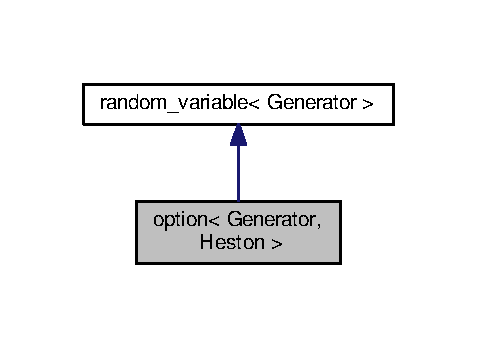
\includegraphics[width=229pt]{classoption__inherit__graph}
\end{center}
\end{figure}


Collaboration diagram for option$<$ Generator, Heston $>$\+:\nopagebreak
\begin{figure}[H]
\begin{center}
\leavevmode
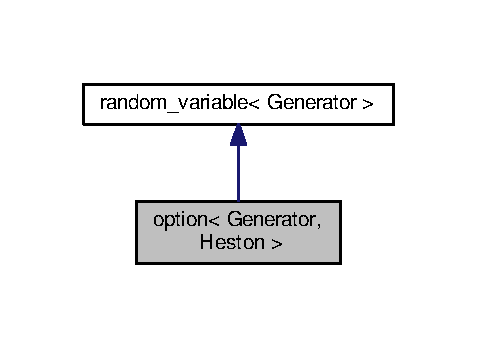
\includegraphics[width=229pt]{classoption__coll__graph}
\end{center}
\end{figure}
\subsection*{Public Member Functions}
\begin{DoxyCompactItemize}
\item 
\hyperlink{classoption_aae400d0330363c992401fd59b6b1e499}{option} ()\hypertarget{classoption_aae400d0330363c992401fd59b6b1e499}{}\label{classoption_aae400d0330363c992401fd59b6b1e499}

\begin{DoxyCompactList}\small\item\em Constructor. \end{DoxyCompactList}\item 
\hyperlink{classoption_aeeb6541a65f9268f3e92cc8d1b1c2d16}{$\sim$option} ()\hypertarget{classoption_aeeb6541a65f9268f3e92cc8d1b1c2d16}{}\label{classoption_aeeb6541a65f9268f3e92cc8d1b1c2d16}

\begin{DoxyCompactList}\small\item\em Destructor. \end{DoxyCompactList}\item 
\hyperlink{classoption_ab2f0aa182faced1a9fa14ebe24485a13}{option} (double maturity, double strike, double cir\+\_\+0, double x\+\_\+0, double a, double k, double sigma, double rho, double r, char type)\hypertarget{classoption_ab2f0aa182faced1a9fa14ebe24485a13}{}\label{classoption_ab2f0aa182faced1a9fa14ebe24485a13}

\begin{DoxyCompactList}\small\item\em Constructor. \end{DoxyCompactList}\item 
double \hyperlink{classoption_aa5cfc4d34a55ab409553af33109099a6}{payoff} (std\+::vector$<$ std\+::vector$<$ double $>$ $>$ trajectory)\hypertarget{classoption_aa5cfc4d34a55ab409553af33109099a6}{}\label{classoption_aa5cfc4d34a55ab409553af33109099a6}

\begin{DoxyCompactList}\small\item\em Computes the payoff of the option given the trajectory of a Heston. \end{DoxyCompactList}\item 
double \hyperlink{classoption_ae1b1d237ddf3d294cf42cdf33eeea7ba}{test\+\_\+log\+\_\+spot\+\_\+one} (std\+::vector$<$ std\+::vector$<$ double $>$ $>$ trajectory)\hypertarget{classoption_ae1b1d237ddf3d294cf42cdf33eeea7ba}{}\label{classoption_ae1b1d237ddf3d294cf42cdf33eeea7ba}

\begin{DoxyCompactList}\small\item\em Function to test log\+\_\+spot\+\_\+one. \end{DoxyCompactList}\item 
double \hyperlink{classoption_a74c39ed0494f2e66bd92ea84bd5dfa4b}{operator()} (Generator \&gen)\hypertarget{classoption_a74c39ed0494f2e66bd92ea84bd5dfa4b}{}\label{classoption_a74c39ed0494f2e66bd92ea84bd5dfa4b}

\begin{DoxyCompactList}\small\item\em Virtual function. \end{DoxyCompactList}\item 
void \hyperlink{classoption_a77b5efa87751a2e506de485483bbd6d8}{set\+\_\+num\+\_\+steps} (unsigned int n)\hypertarget{classoption_a77b5efa87751a2e506de485483bbd6d8}{}\label{classoption_a77b5efa87751a2e506de485483bbd6d8}

\begin{DoxyCompactList}\small\item\em Setter. \end{DoxyCompactList}\item 
double \hyperlink{classoption_a89c94c4ac7adbacbd9e9e667063e78d5}{theoretical\+\_\+log\+\_\+spot\+\_\+one} ()\hypertarget{classoption_a89c94c4ac7adbacbd9e9e667063e78d5}{}\label{classoption_a89c94c4ac7adbacbd9e9e667063e78d5}

\begin{DoxyCompactList}\small\item\em Getter. \end{DoxyCompactList}\item 
std\+::pair$<$ double, double $>$ {\bfseries simulate} (Generator \&gen)\hypertarget{classoption_ab40f18be710881323f35c3589485b602}{}\label{classoption_ab40f18be710881323f35c3589485b602}

\item 
double {\bfseries get\+\_\+mean\+\_\+control\+\_\+variate} ()\hypertarget{classoption_ab19b308a078fdd3812e6cc4f2afe1ec1}{}\label{classoption_ab19b308a078fdd3812e6cc4f2afe1ec1}

\end{DoxyCompactItemize}
\subsection*{Additional Inherited Members}


\subsection{Detailed Description}
\subsubsection*{template$<$typename Generator, typename Heston$>$\\*
class option$<$ Generator, Heston $>$}

A class to code an option. 

The option can be both European or Asian. 

The documentation for this class was generated from the following file\+:\begin{DoxyCompactItemize}
\item 
/home/gregory/\+Desktop/\+Cours\+\_\+\+E\+K/\+P2/\+Pages\+\_\+projet/test\+\_\+git/proba\+\_\+num/src/option.\+h\end{DoxyCompactItemize}

\hypertarget{classprocess}{}\section{process$<$ Generator $>$ Class Template Reference}
\label{classprocess}\index{process$<$ Generator $>$@{process$<$ Generator $>$}}


A general class to code the discretization of a stochastic process on the time interval \mbox{[}0,T\mbox{]}.  




{\ttfamily \#include $<$process.\+h$>$}



Inheritance diagram for process$<$ Generator $>$\+:\nopagebreak
\begin{figure}[H]
\begin{center}
\leavevmode
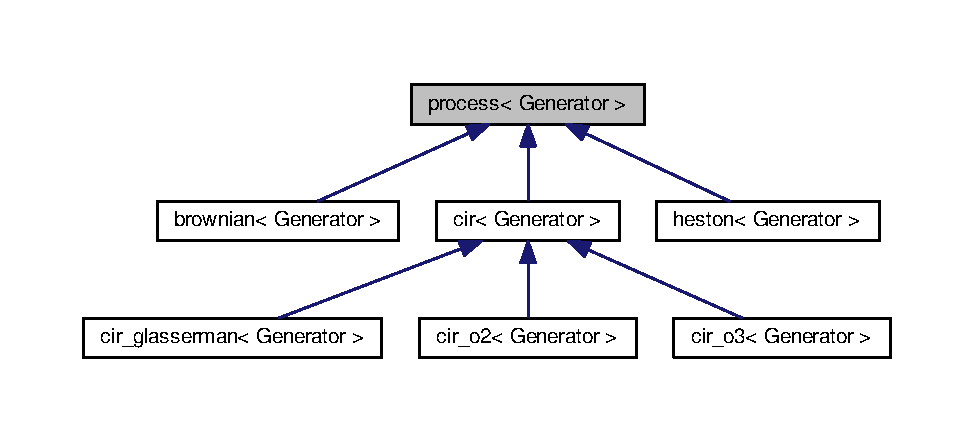
\includegraphics[width=350pt]{classprocess__inherit__graph}
\end{center}
\end{figure}
\subsection*{Public Member Functions}
\begin{DoxyCompactItemize}
\item 
\hyperlink{classprocess_a59faea64773f0619162d80135c334c80}{process} ()\hypertarget{classprocess_a59faea64773f0619162d80135c334c80}{}\label{classprocess_a59faea64773f0619162d80135c334c80}

\begin{DoxyCompactList}\small\item\em Constructor. \end{DoxyCompactList}\item 
\hyperlink{classprocess_af5f38b7ec02665033d47936fec5c498d}{$\sim$process} ()\hypertarget{classprocess_af5f38b7ec02665033d47936fec5c498d}{}\label{classprocess_af5f38b7ec02665033d47936fec5c498d}

\begin{DoxyCompactList}\small\item\em Destructor. \end{DoxyCompactList}\item 
void \hyperlink{classprocess_aaf36acd58fc1d875a6b1ad9e3000c9f9}{set\+\_\+time\+\_\+end} (double t)\hypertarget{classprocess_aaf36acd58fc1d875a6b1ad9e3000c9f9}{}\label{classprocess_aaf36acd58fc1d875a6b1ad9e3000c9f9}

\begin{DoxyCompactList}\small\item\em Setter. \end{DoxyCompactList}\item 
void \hyperlink{classprocess_a479e9c720b3fb9a9e900a1dc6e85b7b8}{set\+\_\+num\+\_\+steps} (unsigned int n)\hypertarget{classprocess_a479e9c720b3fb9a9e900a1dc6e85b7b8}{}\label{classprocess_a479e9c720b3fb9a9e900a1dc6e85b7b8}

\begin{DoxyCompactList}\small\item\em Setter. \end{DoxyCompactList}\item 
void \hyperlink{classprocess_a1c1550dc3afc293860934496a3239a62}{set\+\_\+state\+\_\+0} (std\+::vector$<$ double $>$ s)\hypertarget{classprocess_a1c1550dc3afc293860934496a3239a62}{}\label{classprocess_a1c1550dc3afc293860934496a3239a62}

\begin{DoxyCompactList}\small\item\em Setter. \end{DoxyCompactList}\item 
void \hyperlink{classprocess_af548473ced7827cf2f100a2c74cdaf76}{set\+\_\+time\+\_\+grid} ()\hypertarget{classprocess_af548473ced7827cf2f100a2c74cdaf76}{}\label{classprocess_af548473ced7827cf2f100a2c74cdaf76}

\begin{DoxyCompactList}\small\item\em Setter. \end{DoxyCompactList}\item 
void \hyperlink{classprocess_a149855679fd1188aee51401c07ad35f7}{set\+\_\+state} (std\+::vector$<$ double $>$ s)\hypertarget{classprocess_a149855679fd1188aee51401c07ad35f7}{}\label{classprocess_a149855679fd1188aee51401c07ad35f7}

\begin{DoxyCompactList}\small\item\em Setter. \end{DoxyCompactList}\item 
unsigned int \hyperlink{classprocess_ac469abbf135402311103bf3ca1900748}{get\+\_\+num\+\_\+steps} ()\hypertarget{classprocess_ac469abbf135402311103bf3ca1900748}{}\label{classprocess_ac469abbf135402311103bf3ca1900748}

\begin{DoxyCompactList}\small\item\em Getter. \end{DoxyCompactList}\item 
std\+::vector$<$ double $>$ \hyperlink{classprocess_aef5d6a76efc3aa712f8cd41bf9438cba}{get\+\_\+state\+\_\+0} ()\hypertarget{classprocess_aef5d6a76efc3aa712f8cd41bf9438cba}{}\label{classprocess_aef5d6a76efc3aa712f8cd41bf9438cba}

\begin{DoxyCompactList}\small\item\em Getter. \end{DoxyCompactList}\item 
double \hyperlink{classprocess_a047f0d44f3ec8ddd8d5edfcc09192615}{get\+\_\+time\+\_\+end} ()\hypertarget{classprocess_a047f0d44f3ec8ddd8d5edfcc09192615}{}\label{classprocess_a047f0d44f3ec8ddd8d5edfcc09192615}

\begin{DoxyCompactList}\small\item\em Getter. \end{DoxyCompactList}\item 
double \hyperlink{classprocess_acef251d897e6cec1fe68d1bb59094013}{get\+\_\+time\+\_\+step} ()\hypertarget{classprocess_acef251d897e6cec1fe68d1bb59094013}{}\label{classprocess_acef251d897e6cec1fe68d1bb59094013}

\begin{DoxyCompactList}\small\item\em Getter. \end{DoxyCompactList}\item 
void \hyperlink{classprocess_a5fc8d61bdb3373b5f1a2b123bd8b2556}{write\+\_\+to\+\_\+plot} (Generator \&gen, unsigned int num\+\_\+plots, int coordinate)
\begin{DoxyCompactList}\small\item\em For plotting. \end{DoxyCompactList}\item 
virtual std\+::vector$<$ double $>$ \hyperlink{classprocess_a55c46e4b4ab1992ce09f4133fb484fd6}{next\+\_\+step} (Generator \&gen, std\+::vector$<$ double $>$ state, double t)=0
\begin{DoxyCompactList}\small\item\em Function Next Step. \end{DoxyCompactList}\item 
std\+::vector$<$ std\+::vector$<$ double $>$ $>$ \hyperlink{classprocess_ac728fbbd27c9e9d0b590e18e132480af}{operator()} (Generator \&gen)
\begin{DoxyCompactList}\small\item\em Operator() \end{DoxyCompactList}\item 
void \hyperlink{classprocess_ac74ffbcbb3f61ed3c9b17df1e844e4ee}{print\+\_\+trajectory} (int coordinate)\hypertarget{classprocess_ac74ffbcbb3f61ed3c9b17df1e844e4ee}{}\label{classprocess_ac74ffbcbb3f61ed3c9b17df1e844e4ee}

\begin{DoxyCompactList}\small\item\em Prints the results of the discretization. \end{DoxyCompactList}\end{DoxyCompactItemize}
\subsection*{Protected Attributes}
\begin{DoxyCompactItemize}
\item 
unsigned int {\bfseries dimension}\hypertarget{classprocess_ae6e8422beca0108090a599f2913146f4}{}\label{classprocess_ae6e8422beca0108090a599f2913146f4}

\item 
double \hyperlink{classprocess_a058283b545a3ac9733136b6f48177586}{time\+\_\+step}
\item 
double \hyperlink{classprocess_aee60ec54e570201c8c115005aa0a4f30}{time\+\_\+end}
\item 
unsigned int \hyperlink{classprocess_a90acfc839d6d7465c4aa311bb6970788}{num\+\_\+steps}
\item 
std\+::vector$<$ double $>$ \hyperlink{classprocess_ab4d01c8ea2e9c8285134786d32ae42aa}{state\+\_\+0}
\item 
std\+::vector$<$ double $>$ {\bfseries state}\hypertarget{classprocess_a99c7e9db851147c1bb7142ac0ebb8761}{}\label{classprocess_a99c7e9db851147c1bb7142ac0ebb8761}

\item 
std\+::vector$<$ double $>$ {\bfseries time\+\_\+grid}\hypertarget{classprocess_ac2ac343c501e1a021c83347357730f03}{}\label{classprocess_ac2ac343c501e1a021c83347357730f03}

\item 
std\+::vector$<$ std\+::vector$<$ double $>$ $>$ \hyperlink{classprocess_a63939362bca6b3ee7941c7219954719c}{trajectory}
\item 
bool {\bfseries computed}\hypertarget{classprocess_a9cd553ee907233430f82f82496dfc909}{}\label{classprocess_a9cd553ee907233430f82f82496dfc909}

\end{DoxyCompactItemize}


\subsection{Detailed Description}
\subsubsection*{template$<$typename Generator$>$\\*
class process$<$ Generator $>$}

A general class to code the discretization of a stochastic process on the time interval \mbox{[}0,T\mbox{]}. 

The discretization scheme can be fixed either by chosing the time horizon (time\+\_\+end) or the number of steps (num\+\_\+steps). 

\subsection{Member Function Documentation}
\index{process@{process}!next\+\_\+step@{next\+\_\+step}}
\index{next\+\_\+step@{next\+\_\+step}!process@{process}}
\subsubsection[{\texorpdfstring{next\+\_\+step(\+Generator \&gen, std\+::vector$<$ double $>$ state, double t)=0}{next_step(Generator &gen, std::vector< double > state, double t)=0}}]{\setlength{\rightskip}{0pt plus 5cm}template$<$typename Generator $>$ virtual std\+::vector$<$double$>$ {\bf process}$<$ Generator $>$\+::next\+\_\+step (
\begin{DoxyParamCaption}
\item[{Generator \&}]{gen, }
\item[{std\+::vector$<$ double $>$}]{state, }
\item[{double}]{t}
\end{DoxyParamCaption}
)\hspace{0.3cm}{\ttfamily [pure virtual]}}\hypertarget{classprocess_a55c46e4b4ab1992ce09f4133fb484fd6}{}\label{classprocess_a55c46e4b4ab1992ce09f4133fb484fd6}


Function Next Step. 

Pure virtual function that will be over-\/written for every instance of process. Computes the value of the discretized process at time t + time\+\_\+step. The value of the discretized process at t is stored in state. 

Implemented in \hyperlink{classcir__glasserman_aa3a48d9de6edccd4bfb8a52a5e5ad3df}{cir\+\_\+glasserman$<$ Generator $>$}, \hyperlink{classcir__o3_a77d0f79c0634f1d6cd19017e56eab451}{cir\+\_\+o3$<$ Generator $>$}, \hyperlink{classcir__o2_aff77d63ff38cedf7f720f4bf081b3812}{cir\+\_\+o2$<$ Generator $>$}, \hyperlink{classheston_a81ef826578f2a62320698e88cc2b1b3b}{heston$<$ Generator, Cir $>$}, \hyperlink{classcir_ad3d4f7db1a4448632a6fdbada17cc651}{cir$<$ Generator $>$}, and \hyperlink{classbrownian_afb58e5d64bc76193fcce54cf611f3671}{brownian$<$ Generator $>$}.

\index{process@{process}!operator()@{operator()}}
\index{operator()@{operator()}!process@{process}}
\subsubsection[{\texorpdfstring{operator()(\+Generator \&gen)}{operator()(Generator &gen)}}]{\setlength{\rightskip}{0pt plus 5cm}template$<$typename Generator $>$ std\+::vector$<$ std\+::vector$<$ double $>$ $>$ {\bf process}$<$ Generator $>$\+::operator() (
\begin{DoxyParamCaption}
\item[{Generator \&}]{gen}
\end{DoxyParamCaption}
)}\hypertarget{classprocess_ac728fbbd27c9e9d0b590e18e132480af}{}\label{classprocess_ac728fbbd27c9e9d0b590e18e132480af}


Operator() 

Overloads the operator (). Allows to draw a new instance of the discretized process. \index{process@{process}!write\+\_\+to\+\_\+plot@{write\+\_\+to\+\_\+plot}}
\index{write\+\_\+to\+\_\+plot@{write\+\_\+to\+\_\+plot}!process@{process}}
\subsubsection[{\texorpdfstring{write\+\_\+to\+\_\+plot(\+Generator \&gen, unsigned int num\+\_\+plots, int coordinate)}{write_to_plot(Generator &gen, unsigned int num_plots, int coordinate)}}]{\setlength{\rightskip}{0pt plus 5cm}template$<$typename Generator $>$ void {\bf process}$<$ Generator $>$\+::write\+\_\+to\+\_\+plot (
\begin{DoxyParamCaption}
\item[{Generator \&}]{gen, }
\item[{unsigned int}]{num\+\_\+plots, }
\item[{int}]{coordinate}
\end{DoxyParamCaption}
)}\hypertarget{classprocess_a5fc8d61bdb3373b5f1a2b123bd8b2556}{}\label{classprocess_a5fc8d61bdb3373b5f1a2b123bd8b2556}


For plotting. 

Computes and plots num\+\_\+plot instances of the discretized process. The method writes the relevant data in a .dat file and calls gnuplot for plotting 

\subsection{Member Data Documentation}
\index{process@{process}!num\+\_\+steps@{num\+\_\+steps}}
\index{num\+\_\+steps@{num\+\_\+steps}!process@{process}}
\subsubsection[{\texorpdfstring{num\+\_\+steps}{num_steps}}]{\setlength{\rightskip}{0pt plus 5cm}template$<$typename Generator $>$ unsigned int {\bf process}$<$ Generator $>$\+::num\+\_\+steps\hspace{0.3cm}{\ttfamily [protected]}}\hypertarget{classprocess_a90acfc839d6d7465c4aa311bb6970788}{}\label{classprocess_a90acfc839d6d7465c4aa311bb6970788}
Number of steps in time discretization \index{process@{process}!state\+\_\+0@{state\+\_\+0}}
\index{state\+\_\+0@{state\+\_\+0}!process@{process}}
\subsubsection[{\texorpdfstring{state\+\_\+0}{state_0}}]{\setlength{\rightskip}{0pt plus 5cm}template$<$typename Generator $>$ std\+::vector$<$double$>$ {\bf process}$<$ Generator $>$\+::state\+\_\+0\hspace{0.3cm}{\ttfamily [protected]}}\hypertarget{classprocess_ab4d01c8ea2e9c8285134786d32ae42aa}{}\label{classprocess_ab4d01c8ea2e9c8285134786d32ae42aa}
Initial value for the process at time t = 0 \index{process@{process}!time\+\_\+end@{time\+\_\+end}}
\index{time\+\_\+end@{time\+\_\+end}!process@{process}}
\subsubsection[{\texorpdfstring{time\+\_\+end}{time_end}}]{\setlength{\rightskip}{0pt plus 5cm}template$<$typename Generator $>$ double {\bf process}$<$ Generator $>$\+::time\+\_\+end\hspace{0.3cm}{\ttfamily [protected]}}\hypertarget{classprocess_aee60ec54e570201c8c115005aa0a4f30}{}\label{classprocess_aee60ec54e570201c8c115005aa0a4f30}
Simulation between 0 and time\+\_\+end \index{process@{process}!time\+\_\+step@{time\+\_\+step}}
\index{time\+\_\+step@{time\+\_\+step}!process@{process}}
\subsubsection[{\texorpdfstring{time\+\_\+step}{time_step}}]{\setlength{\rightskip}{0pt plus 5cm}template$<$typename Generator $>$ double {\bf process}$<$ Generator $>$\+::time\+\_\+step\hspace{0.3cm}{\ttfamily [protected]}}\hypertarget{classprocess_a058283b545a3ac9733136b6f48177586}{}\label{classprocess_a058283b545a3ac9733136b6f48177586}
Time step of the discretization \index{process@{process}!trajectory@{trajectory}}
\index{trajectory@{trajectory}!process@{process}}
\subsubsection[{\texorpdfstring{trajectory}{trajectory}}]{\setlength{\rightskip}{0pt plus 5cm}template$<$typename Generator $>$ std\+::vector$<$std\+::vector$<$double$>$ $>$ {\bf process}$<$ Generator $>$\+::trajectory\hspace{0.3cm}{\ttfamily [protected]}}\hypertarget{classprocess_a63939362bca6b3ee7941c7219954719c}{}\label{classprocess_a63939362bca6b3ee7941c7219954719c}
Vector of vectors used to compute the values taken by the process This choice is motivated by the mutli-\/dimensional Heston model 

The documentation for this class was generated from the following file\+:\begin{DoxyCompactItemize}
\item 
/home/gregory/\+Desktop/\+Cours\+\_\+\+E\+K/\+P2/\+Pages\+\_\+projet/test\+\_\+git/proba\+\_\+num/src/process.\+h\end{DoxyCompactItemize}

\hypertarget{classrademacher}{}\section{rademacher$<$ Generator $>$ Class Template Reference}
\label{classrademacher}\index{rademacher$<$ Generator $>$@{rademacher$<$ Generator $>$}}


A Rademacher random variable.  




{\ttfamily \#include $<$normal.\+h$>$}



Inheritance diagram for rademacher$<$ Generator $>$\+:\nopagebreak
\begin{figure}[H]
\begin{center}
\leavevmode
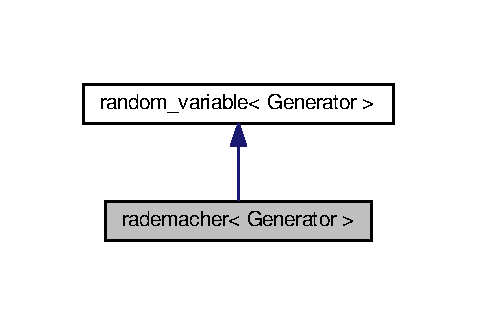
\includegraphics[width=229pt]{classrademacher__inherit__graph}
\end{center}
\end{figure}


Collaboration diagram for rademacher$<$ Generator $>$\+:\nopagebreak
\begin{figure}[H]
\begin{center}
\leavevmode
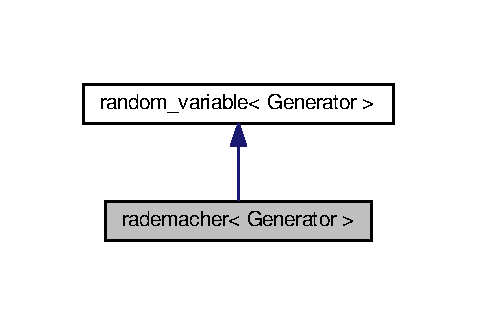
\includegraphics[width=229pt]{classrademacher__coll__graph}
\end{center}
\end{figure}
\subsection*{Public Member Functions}
\begin{DoxyCompactItemize}
\item 
double \hyperlink{classrademacher_ad497f5af40bc0d18d33d04c9e13976c1}{operator()} (Generator \&gen)\hypertarget{classrademacher_ad497f5af40bc0d18d33d04c9e13976c1}{}\label{classrademacher_ad497f5af40bc0d18d33d04c9e13976c1}

\begin{DoxyCompactList}\small\item\em Virtual function. \end{DoxyCompactList}\end{DoxyCompactItemize}
\subsection*{Additional Inherited Members}


\subsection{Detailed Description}
\subsubsection*{template$<$typename Generator$>$\\*
class rademacher$<$ Generator $>$}

A Rademacher random variable. 

The documentation for this class was generated from the following file\+:\begin{DoxyCompactItemize}
\item 
/home/gregory/\+Desktop/\+Cours\+\_\+\+E\+K/\+P2/\+Pages\+\_\+projet/test\+\_\+git/proba\+\_\+num/src/normal.\+h\end{DoxyCompactItemize}

\hypertarget{classrandom__variable}{}\section{random\+\_\+variable$<$ Generator $>$ Class Template Reference}
\label{classrandom__variable}\index{random\+\_\+variable$<$ Generator $>$@{random\+\_\+variable$<$ Generator $>$}}


A general class to implement a random variable.  




{\ttfamily \#include $<$random\+\_\+variable.\+h$>$}



Inheritance diagram for random\+\_\+variable$<$ Generator $>$\+:\nopagebreak
\begin{figure}[H]
\begin{center}
\leavevmode
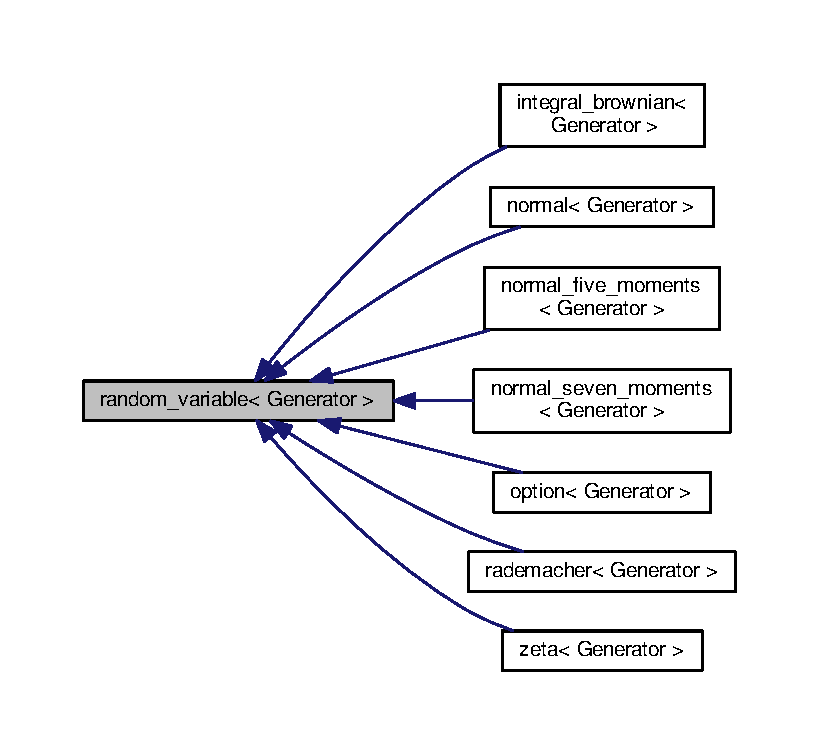
\includegraphics[width=350pt]{classrandom__variable__inherit__graph}
\end{center}
\end{figure}
\subsection*{Public Member Functions}
\begin{DoxyCompactItemize}
\item 
\hyperlink{classrandom__variable_a6dbf2b284fff6629a1bf61ed5f63b1db}{random\+\_\+variable} ()\hypertarget{classrandom__variable_a6dbf2b284fff6629a1bf61ed5f63b1db}{}\label{classrandom__variable_a6dbf2b284fff6629a1bf61ed5f63b1db}

\begin{DoxyCompactList}\small\item\em Constructor. \end{DoxyCompactList}\item 
\hyperlink{classrandom__variable_ae9066f6c557c9b64233f087bd2dfb6b1}{$\sim$random\+\_\+variable} ()\hypertarget{classrandom__variable_ae9066f6c557c9b64233f087bd2dfb6b1}{}\label{classrandom__variable_ae9066f6c557c9b64233f087bd2dfb6b1}

\begin{DoxyCompactList}\small\item\em Destructor. \end{DoxyCompactList}\item 
void \hyperlink{classrandom__variable_aa3b0e1dfeb750216df2043e96f72c017}{print} ()\hypertarget{classrandom__variable_aa3b0e1dfeb750216df2043e96f72c017}{}\label{classrandom__variable_aa3b0e1dfeb750216df2043e96f72c017}

\begin{DoxyCompactList}\small\item\em Printing. \end{DoxyCompactList}\item 
virtual double \hyperlink{classrandom__variable_a661cc29297837ef5aba0b7e476f114b2}{operator()} (Generator \&gen)=0\hypertarget{classrandom__variable_a661cc29297837ef5aba0b7e476f114b2}{}\label{classrandom__variable_a661cc29297837ef5aba0b7e476f114b2}

\begin{DoxyCompactList}\small\item\em Virtual function. \end{DoxyCompactList}\item 
virtual std\+::pair$<$ double, double $>$ {\bfseries simulate} (Generator \&gen)\hypertarget{classrandom__variable_adc681ee20a16d59d75288c4faa969a50}{}\label{classrandom__variable_adc681ee20a16d59d75288c4faa969a50}

\item 
double {\bfseries get\+\_\+mean\+\_\+control\+\_\+variate} ()\hypertarget{classrandom__variable_a1ece3619941def5190b80fd0153e4ef6}{}\label{classrandom__variable_a1ece3619941def5190b80fd0153e4ef6}

\item 
bool {\bfseries has\+\_\+control} ()\hypertarget{classrandom__variable_afae88ea0382990482784b3e16bbb6013}{}\label{classrandom__variable_afae88ea0382990482784b3e16bbb6013}

\end{DoxyCompactItemize}
\subsection*{Protected Attributes}
\begin{DoxyCompactItemize}
\item 
bool {\bfseries realised}\hypertarget{classrandom__variable_a94420df0549a9276fa277e55cd9f8a5c}{}\label{classrandom__variable_a94420df0549a9276fa277e55cd9f8a5c}

\item 
double {\bfseries realisation}\hypertarget{classrandom__variable_a5b1d23131a974247dad648dd36c90732}{}\label{classrandom__variable_a5b1d23131a974247dad648dd36c90732}

\item 
bool {\bfseries has\+\_\+control\+\_\+variate}\hypertarget{classrandom__variable_a0ef52eaf585e41eba031152727eddffa}{}\label{classrandom__variable_a0ef52eaf585e41eba031152727eddffa}

\item 
double {\bfseries control\+\_\+variate\+\_\+realisation}\hypertarget{classrandom__variable_afdb60c3268e929b2878fb71576e9544e}{}\label{classrandom__variable_afdb60c3268e929b2878fb71576e9544e}

\item 
double {\bfseries control\+\_\+variate\+\_\+mean}\hypertarget{classrandom__variable_abeb7535675f902615adda823bb6786cd}{}\label{classrandom__variable_abeb7535675f902615adda823bb6786cd}

\end{DoxyCompactItemize}


\subsection{Detailed Description}
\subsubsection*{template$<$typename Generator$>$\\*
class random\+\_\+variable$<$ Generator $>$}

A general class to implement a random variable. 

The documentation for this class was generated from the following file\+:\begin{DoxyCompactItemize}
\item 
/home/gregory/\+Desktop/\+Cours\+\_\+\+E\+K/\+P2/\+Pages\+\_\+projet/test\+\_\+git/proba\+\_\+num/src/random\+\_\+variable.\+h\end{DoxyCompactItemize}

\hypertarget{classsobol__generator}{}\section{sobol\+\_\+generator Class Reference}
\label{classsobol__generator}\index{sobol\+\_\+generator@{sobol\+\_\+generator}}
\subsection*{Public Member Functions}
\begin{DoxyCompactItemize}
\item 
double {\bfseries operator()} ()\hypertarget{classsobol__generator_aa7956ddb88f92e8ca4b161ae68ce5ec9}{}\label{classsobol__generator_aa7956ddb88f92e8ca4b161ae68ce5ec9}

\item 
double {\bfseries min} ()\hypertarget{classsobol__generator_a31ab8182187885f740e5e05cf889af1d}{}\label{classsobol__generator_a31ab8182187885f740e5e05cf889af1d}

\item 
double {\bfseries max} ()\hypertarget{classsobol__generator_ab22cef51f007246f39754d55a287e70f}{}\label{classsobol__generator_ab22cef51f007246f39754d55a287e70f}

\end{DoxyCompactItemize}


The documentation for this class was generated from the following file\+:\begin{DoxyCompactItemize}
\item 
/home/gregory/\+Desktop/\+Cours\+\_\+\+E\+K/\+P2/\+Pages\+\_\+projet/test\+\_\+git/proba\+\_\+num/src/sobol\+\_\+generator.\+h\end{DoxyCompactItemize}

\hypertarget{classzeta}{}\section{zeta$<$ Generator $>$ Class Template Reference}
\label{classzeta}\index{zeta$<$ Generator $>$@{zeta$<$ Generator $>$}}


A uniform random variable on \{1,2,3\}.  




{\ttfamily \#include $<$normal.\+h$>$}

Inheritance diagram for zeta$<$ Generator $>$\+:\begin{figure}[H]
\begin{center}
\leavevmode
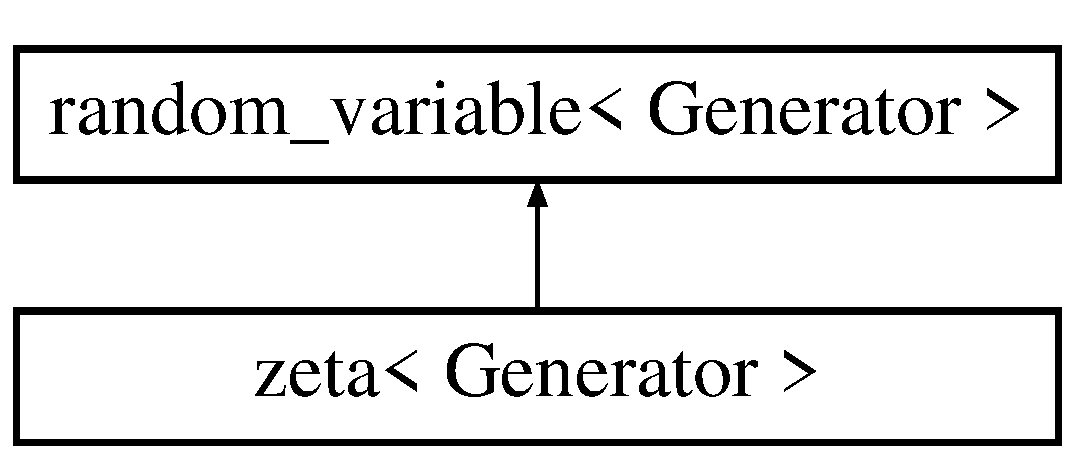
\includegraphics[height=2.000000cm]{classzeta}
\end{center}
\end{figure}
\subsection*{Public Member Functions}
\begin{DoxyCompactItemize}
\item 
\mbox{\Hypertarget{classzeta_ad4df70f32566a510f6e4201f722df570}\label{classzeta_ad4df70f32566a510f6e4201f722df570}} 
double \mbox{\hyperlink{classzeta_ad4df70f32566a510f6e4201f722df570}{operator()}} (Generator \&gen)
\begin{DoxyCompactList}\small\item\em Virtual function. \end{DoxyCompactList}\end{DoxyCompactItemize}
\subsection*{Additional Inherited Members}


\subsection{Detailed Description}
\subsubsection*{template$<$typename Generator$>$\newline
class zeta$<$ Generator $>$}

A uniform random variable on \{1,2,3\}. 

The documentation for this class was generated from the following file\+:\begin{DoxyCompactItemize}
\item 
normal.\+h\end{DoxyCompactItemize}

%--- End generated contents ---

% Index
\backmatter
\newpage
\phantomsection
\clearemptydoublepage
\addcontentsline{toc}{chapter}{Index}
\printindex

\end{document}
